\newcommand{\sketchname}{InterestSketch}

\newcommand{\freCM}{CM with heap}
\newcommand{\freCU}{CM-CU with heap}
\newcommand{\freSS}{SS}
\newcommand{\freCF}{SS with CF}
\newcommand{\freunbia}{Unbiased SS}

\newcommand{\perpie}{PIE}
\newcommand{\perss}{Small-Space}

\newcommand{\supolf}{OLF}
\newcommand{\suptlf}{TLF}
\newcommand{\supopen}{OpenSketch}

\newcommand{\chafr}{FR}
\newcommand{\chafrcf}{FR with CF}

\newcommand{\secss}{using Stream-Summary}
\newcommand{\secmin}{using min-heap}
\newcommand{\secarr}{using Multi-Array}

\newcommand{\taskone}{Frequent Items}
\newcommand{\tasktwo}{Super-Spreaders}
\newcommand{\taskthree}{Persistent Items}
\newcommand{\taskfour}{Heavy Changes}
\newcommand{\taskpara}{Different Versions}

\presec
\section{Experimental Results} \postsec
\label{sec:experiments}

In this section, we provide experimental results where we compare the final version of \sketchname{} with the state-of-the-art algorithms for different definition of interests. Due to space limitation, the experimental figures on AAE and CR are provided in Appendix \ref{app:fig}. Experimental results of comparing different versions of InterestSketch are provided in the end of our technical report \cite{opensource} without identifying information.
%After introducing the experimental setup in Section~\ref{subsec:setup}, we provide results for finding \taskone {} (Section~\ref{eva_one}), \taskfour{} (Section~\ref{eva_four}), \tasktwo {} (Section~\ref{eva_two}), and \taskthree {} (Section~\ref{eva_three}), respectively.
%Finally, we compare different versions of \sketchname{} in Appendix~\ref{eva_para}.
\begin{figure*}[!ht]
	\centering
	%
	\subfigure[Synthetic dataset]{
		\begin{minipage}[t]{0.245\textwidth}{
		\prefig
		\begin{center}
		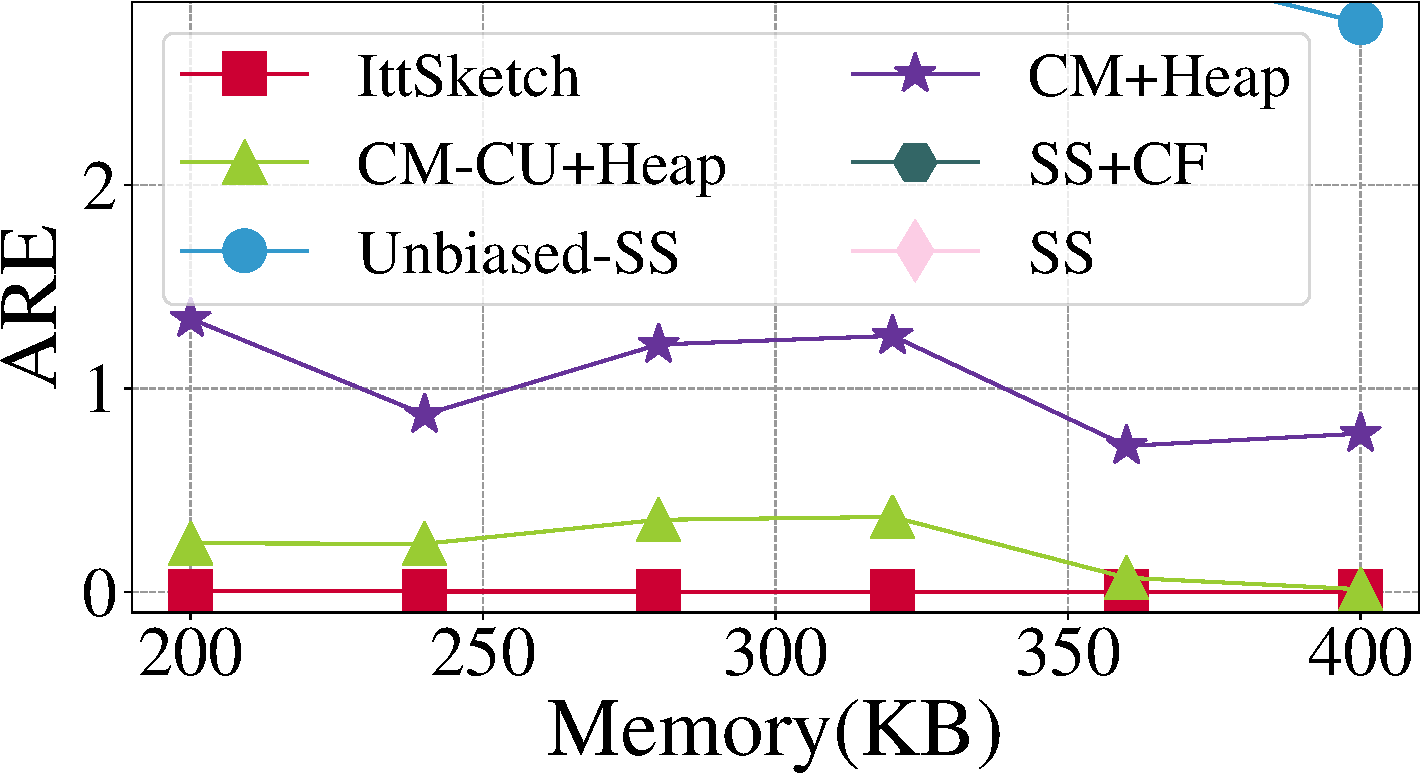
\includegraphics[width=0.95\textwidth, ]{Figures/fre/fre_are/fre_syn_are-cropped.pdf}
		\end{center}
		}
		\postfig 
		\adjustfigs
		\prefigcaption
		\label{fre_are_syn}
		\postfigcaption
		\end{minipage}
	}
	%
	\subfigure[IP trace]{
		\begin{minipage}[t]{0.23\textwidth}{
		\prefig
		\begin{center}
		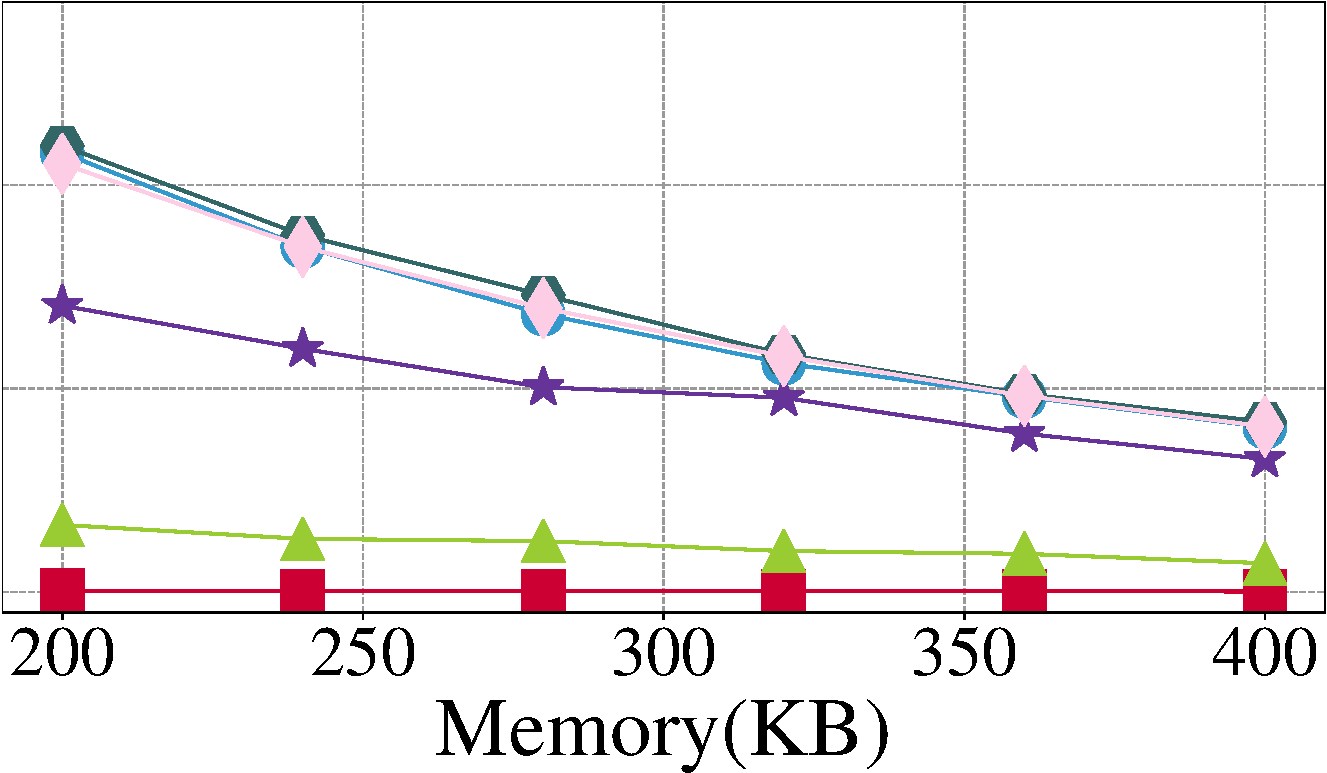
\includegraphics[width=0.95\textwidth, ]{Figures/fre/fre_are/fre_ip_are-cropped.pdf}
		\end{center}
		}
		\postfig
		\adjustfigs
		\prefigcaption
		\label{fre_are_ip}
		\postfigcaption
		\end{minipage}
	}
	%
	\subfigure[Web page]{
		\begin{minipage}[t]{0.23\textwidth}{
		\prefig
		\begin{center}		
		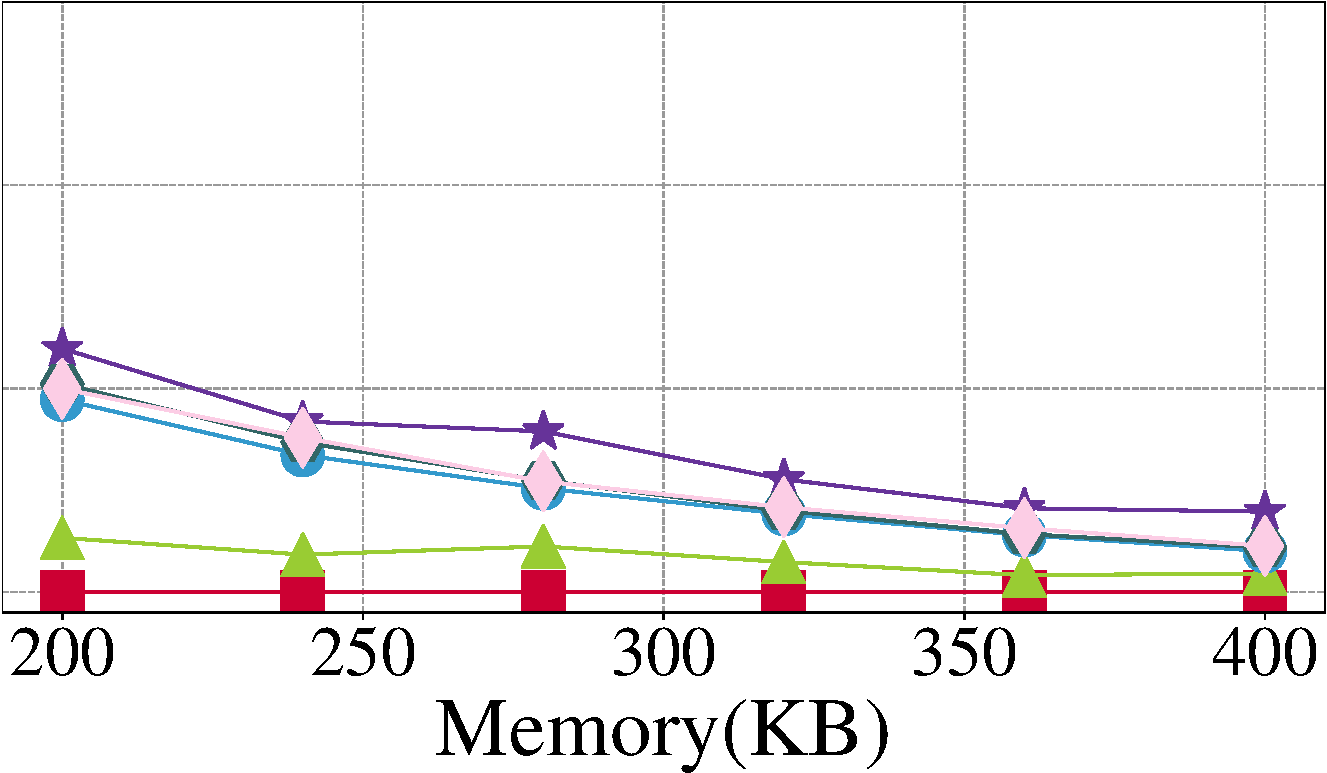
\includegraphics[width=0.95\textwidth, ]{Figures/fre/fre_are/fre_web_are-cropped.pdf}
		\end{center}
		}
	    \postfig 
	    \adjustfigs
	    \prefigcaption
		\label{fre_are_web}
		\postfigcaption
		\end{minipage}
	}
	%
	\subfigure[Network dataset]{
		\begin{minipage}[t]{0.23\textwidth}{
		\prefig
		\begin{center}		
		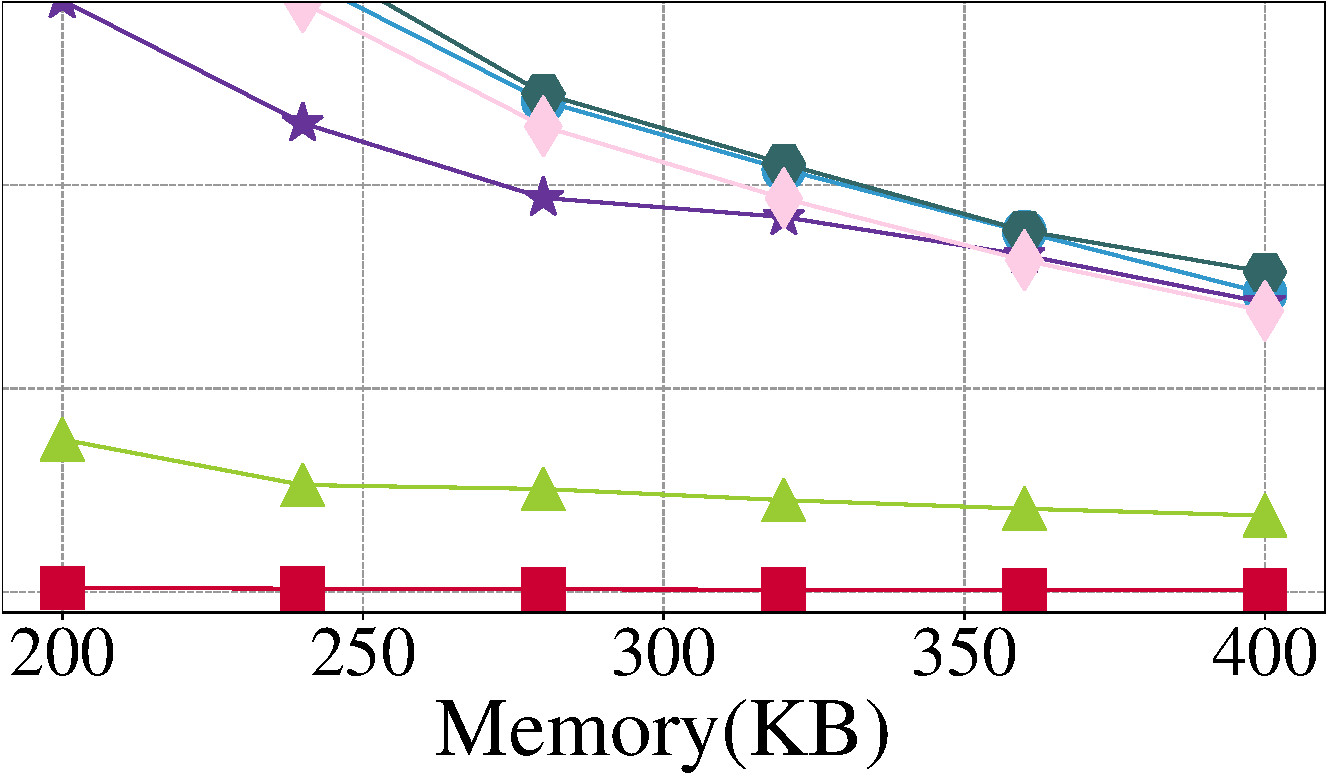
\includegraphics[width=0.95\textwidth, ]{Figures/fre/fre_are/fre_net_are-cropped.pdf}
		\end{center}
		}
		\postfig 
		\adjustfigs
		\prefigcaption
		\label{fre_are_net}
		\postfigcaption
		\end{minipage}
	}
	%
	\vvv \vvv
	\caption{ARE of finding \taskone.}
	\label{fre_are}
\end{figure*}
			
\begin{figure*}[!ht]
	\centering
	%
	\subfigure[Synthetic dataset]{
		\begin{minipage}[t]{0.255\textwidth}{
		\prefig
		\begin{center}
		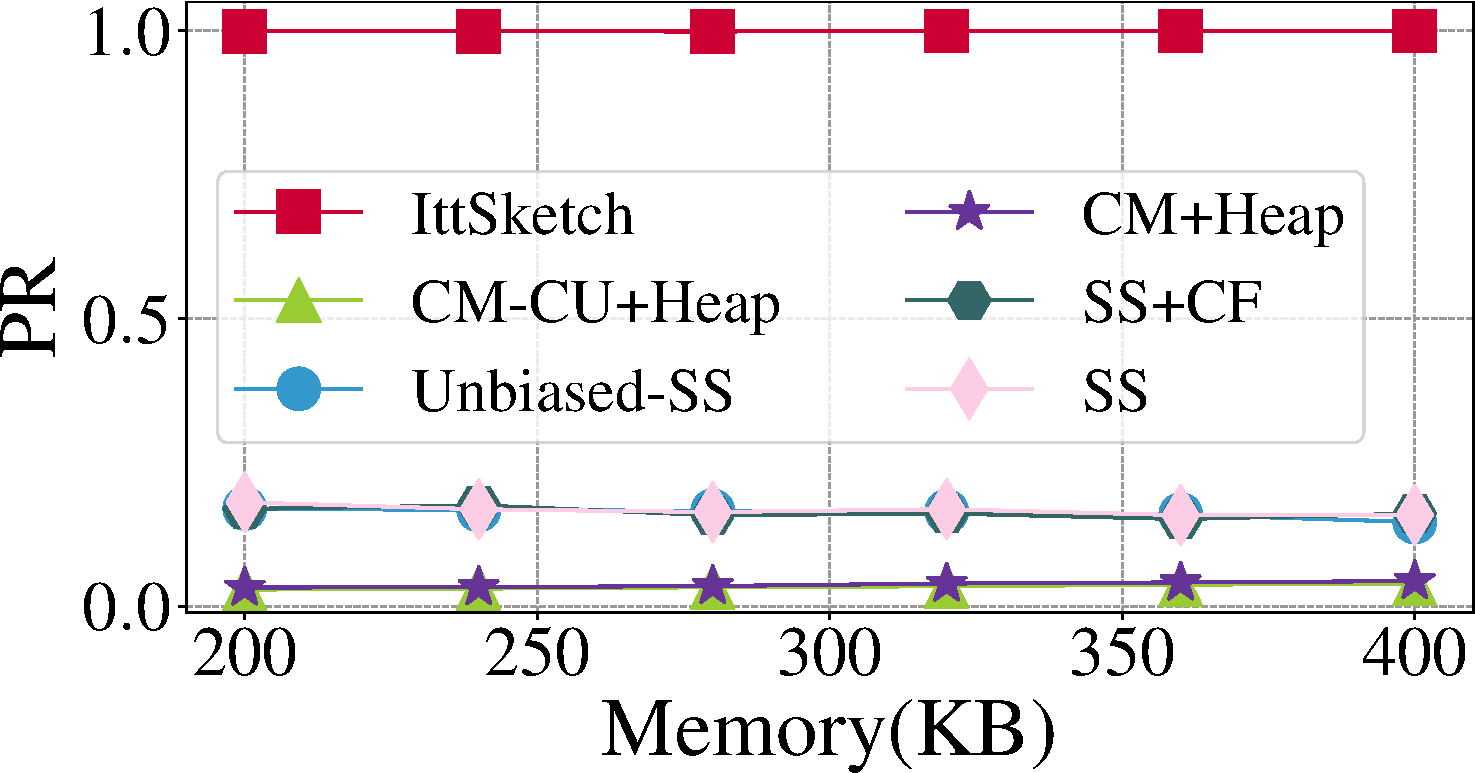
\includegraphics[width=0.95\textwidth, ]{Figures/fre/fre_pr/fre_syn_pr-cropped.pdf}
		\end{center}
		}
		\postfig 
		\adjustfigs
		\prefigcaption
		\label{fre_pr_syn}
		\postfigcaption
		\end{minipage}
	}
	%
	\subfigure[IP trace]{
		\begin{minipage}[t]{0.23\textwidth}{
		\prefig
		\begin{center}
		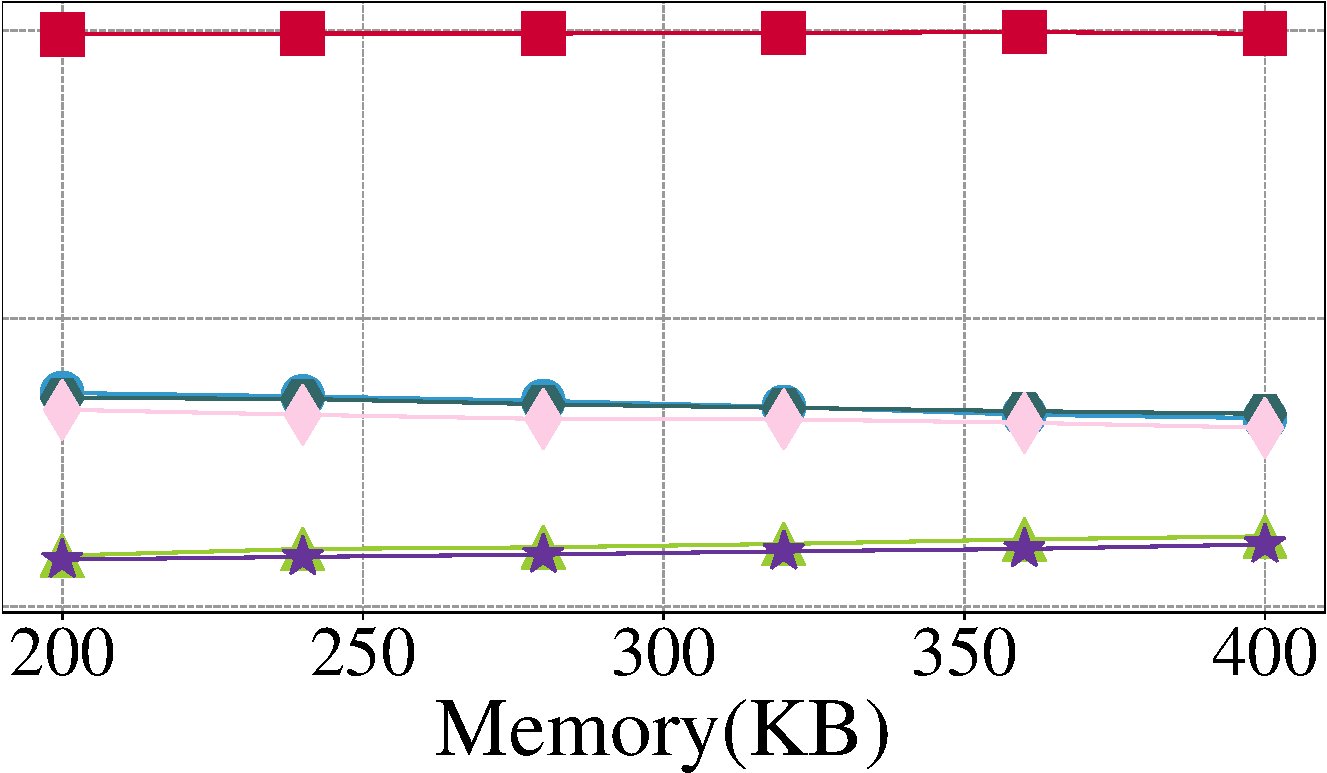
\includegraphics[width=0.95\textwidth, ]{Figures/fre/fre_pr/fre_ip_pr-cropped.pdf}
		\end{center}
		}
		\postfig
		\adjustfigs
		\prefigcaption
		\label{fre_pr_ip}
		\postfigcaption
		\end{minipage}
	}
	%
	\subfigure[Web page]{
		\begin{minipage}[t]{0.23\textwidth}{
		\prefig
		\begin{center}		
		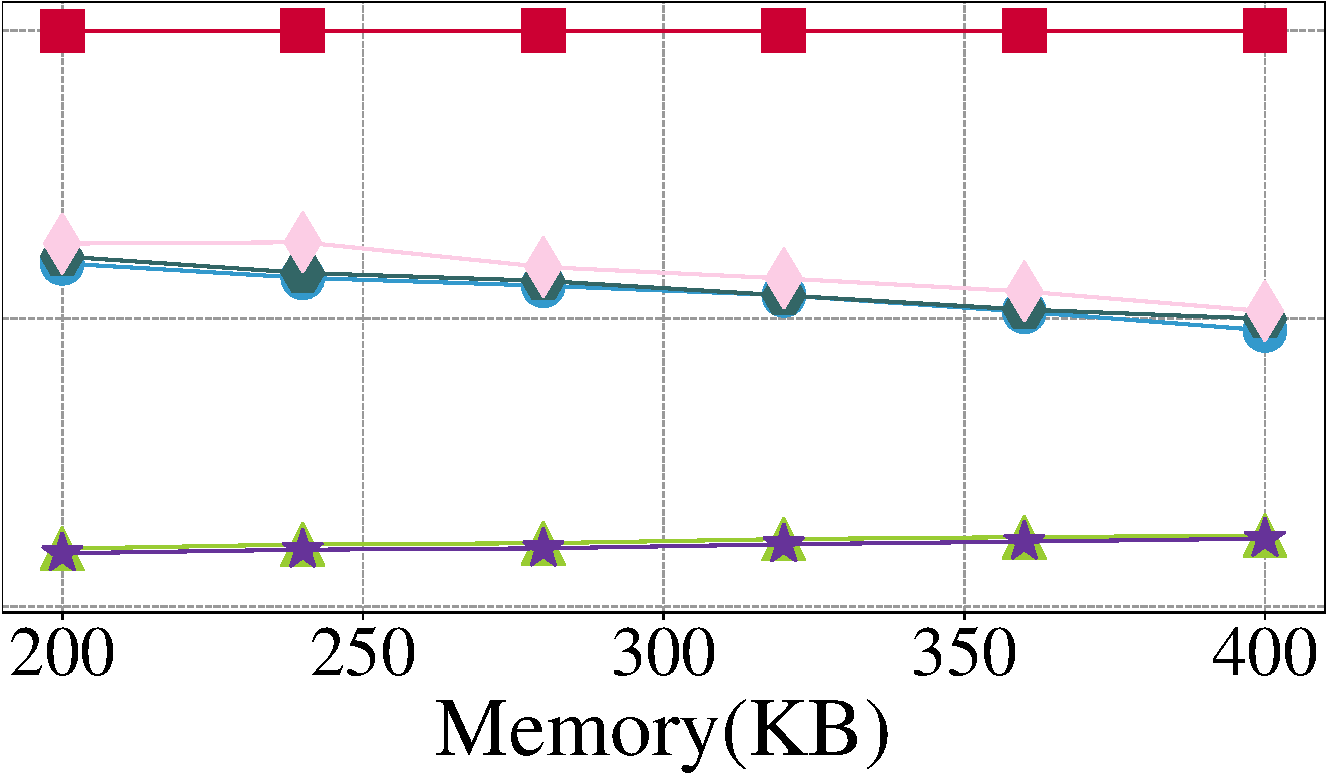
\includegraphics[width=0.95\textwidth, ]{Figures/fre/fre_pr/fre_web_pr-cropped.pdf}
		\end{center}
		}
		\postfig 
		\adjustfigs
		\prefigcaption
		\label{fre_pr_web}
		\postfigcaption
		\end{minipage}
	}
	%
	\subfigure[Network dataset]{
		\begin{minipage}[t]{0.23\textwidth}{
		\prefig
	    \begin{center}		
		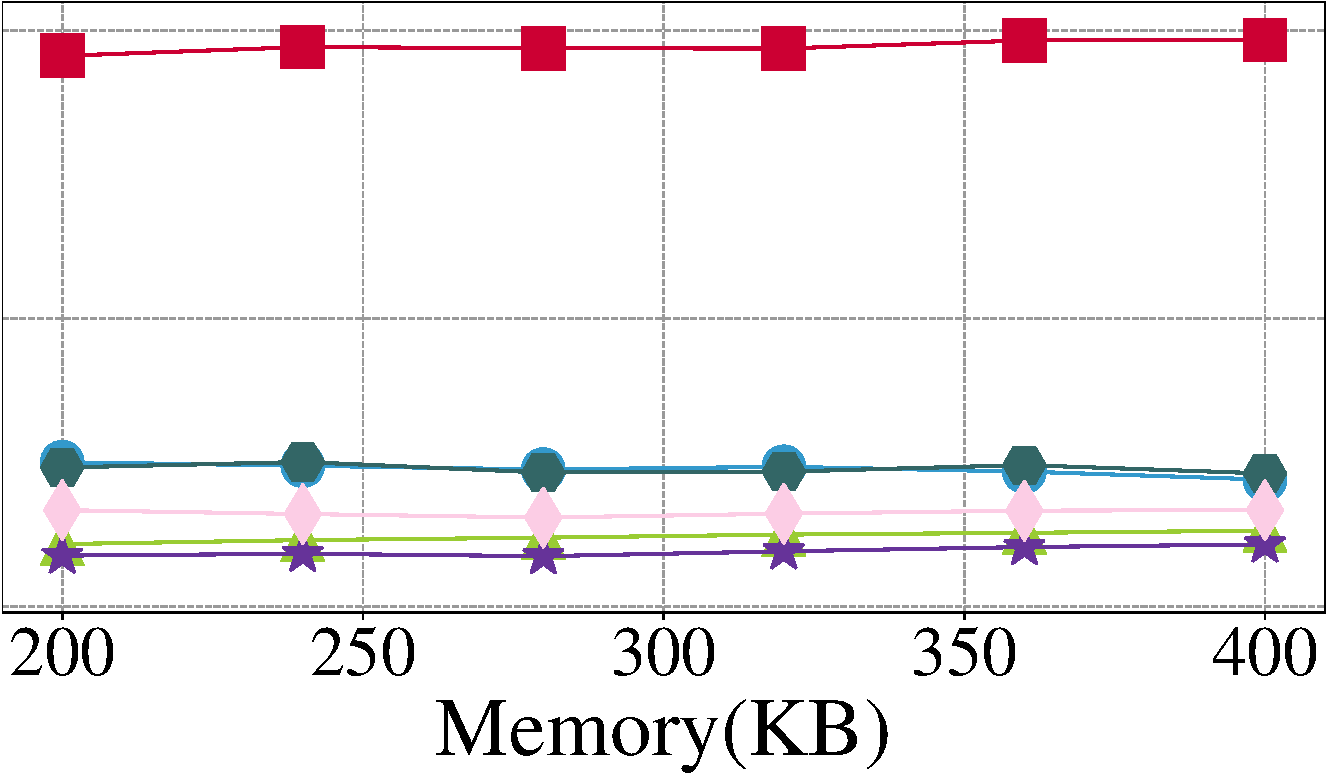
\includegraphics[width=0.95\textwidth, ]{Figures/fre/fre_pr/fre_net_pr-cropped.pdf}
		\end{center}
		}
		\postfig 
		\adjustfigs
		\prefigcaption
		\label{fre_pr_net}
		\postfigcaption
		\end{minipage}
	}
	%
	\vvv \vvv
    \caption{PR of finding \taskone.}
	\label{fre_pr}
\end{figure*}

\presub
\subsection{Experimental Setup} \postsub
\label{subsec:setup}
%
\noindent\textbf{Datasets:}

\noindent\textbf{1) IP Trace Dataset:}
The IP Trace Dataset are streams of anonymized IP traces collected in 2016 by CAIDA~\cite{caida}. Each item contains a source IP address ($4$ bytes) and a destination IP address ($4$ bytes){\color{reviewA} , 8 bytes in total.} {\color{reviewA} For this and the following three datasets, we assume that each item appears at most $2^{32}-1$ times.}

\noindent\textbf{2) Web Page Dataset:}
The Web page dataset is built from a collection of web pages, which were downloaded from the website~\cite{webdocs}.
Each item ($4$ bytes) represents the number of distinct terms in a web page.

\noindent\textbf{3) Synthetic Datasets:}
We generate 10 synthetic datasets which follow the Zipf~\cite{zipf} distribution by using Web Polygraph~\cite{webpoly}, an open source performance testing tool. Each dataset has 32 million items and the skewness of datasets varies from 0.3 to 3.0. The length of each item ID is $4$ bytes. 
In the following experiment, we use the dataset with skewness of 1.5 as synthetic dataset.

\noindent\textbf{4) Network Dataset:}
%This is a temporal network of interactions on the stack exchange web site \cite{net_dat}. Each item consists of three values $u,v,t$, which means user $u$ answered user $v'$s question at time t. We regard $u$ as an item ID and $t$ as its timestamp.
The network dataset contains users' posting history on the stack exchange website~\cite{net_dat}. Each item has three values $u,v,t$, that mean user $u$ answered user $v$'s question at time $t$. We use $u$ as the ID and $t$ as the time stamp of an item.

\noindent\textbf{Implementation:}
We have implemented \sketchname {} in C++.
The hash functions are implemented using the 32-bit Bob Hash (obtained from the open source website~\cite{bobhash}) with different initial seeds. The random function is implemented from the random library in C++. We produce the random number by using the random\_device from the <random> header file of the C++ standard library. All of the abbreviations used in the evaluation and their full name are shown in Table~\ref{abbr}.

\noindent\textbf{Computation Platform:}
We conducted all experiments on a machine with a 2-core processor (4 threads, 6th Gen Intel Core i7-6600U @2.60 GHz)
and 16 GB DRAM memory.
The processor has three levels of cache: one 128KB L1 cache, one 512KB L2 cache, and one 4MB L3 cache. 

\noindent\textbf{Metrics:}
\label{subsec:eva:metric}

%We use the following metrics (including accuracy metrics and insertion speed) to evaluate the performance of our algorithms. In experiment, we discover that after reading enough items (usually $1\sim2$ window sizes), the experiment result  will become stable. We measure the metrics in different window (after the first window), and compute the average value. We use the average value to represent the experiment result at given parameter setting. The error bar represents the minimal value and the maximum value.%

\noindent\textbf{1) Average Absolute Error (AAE):} $\frac{1}{|\mathbf{\Psi}|} \sum_{e_i \in \mathbf{\Psi}}|\iii_i-\widehat{\iii_i}| $,
where $\iii_i$ is the real interest of item $e_i$, $\widehat{\iii_i}$ is its estimated interest, and $\mathbf{\Psi}$ is the query set. 
Here, we query the dataset by querying every distinct item once in the sketch.

\noindent\textbf{2) Average Relative Error (ARE):} $\frac{1}{|\mathbf{\Psi}|} \sum_{e_i \in \mathbf{\Psi}}|\iii_i-\widehat{\iii_i}|/ \iii_i $,
where $\iii_i$ is the real interest of item $e_i$, $\widehat{\iii_i}$ is its estimated interest, and $\mathbf{\Psi}$ is the query set. 
Here, we query the dataset by querying each correct instance once in the sketch.

\noindent\textbf{3) Precision Rate (PR):}
Ratio of the number of correctly reported items to the number of reported items.

\noindent\textbf{4) Recall Rate (CR):}
Ratio of the number of correctly reported items to the number of correct items.

\noindent\textbf{5) Speed:}
Million operations (insertions) per second (Mops).
All the experiments about speed are repeated 10 times and the average speed is reported.

{\color{reviewD}
\noindent\textbf{6) Latency:}
Average process time needed by each item.
}

% Steve: a reviewer might want to see the standard deviation as well...

Let $d$ be the number of cells in each bucket. For our \sketchname{} in the following experiments, we set $d=8$.

\begin{table}
\vspace{-0.05in}
\caption{Abbreviations in experiment}
\vspace{-0.1in}
\label{abbr}
\begin{tabular}{|c|l|}
\hline
Abbreviation&Full name\\
\hline
CM&Count-Min Sketch\cite{cmsketch}\\
\hline
FR&Flow\cite{flowradar}\\
\hline
SS&SpaceSaving\cite{spacesaving}\\
\hline
CF&Cold Filter\cite{coldfilter}\\
\hline
OLF&One-level Filtering\cite{superspreader}\\  
\hline
TLF&Two-level Filtering\cite{superspreader}\\
\hline
SHF&Second Half First\\
\hline
IttSketch&The final version of \sketchname{} in \S \ref{sec:final}\\
\hline
\end{tabular}
\end{table}
\presub
\subsection{Evaluation on Finding \taskone} \postsub
\label{eva_one}

\noindent\textbf{Parameter Setting:}
%We compare three frameworks: \sketchname, \EHname and \Splittername. For each frameworks, we using CM Sketch, CM-CU Sketch and Count Sketch approaches.
%
%We compare 5 approaches: CM \sketchname, CM-CU \sketchname, Count \sketchname, \EHname {} and \Splittername.
%
We compare 6 algorithms: \sketchname, \freCM\cite{cmsketch}, \freCU\cite{cusketch}, \freCF\cite{coldfilter}, \freSS\cite{spacesaving}, and \freunbia\cite{unbiasedsketch}.
For \freCM, \freCU{}, and \freCF, the parameters are set according to the recommendation of the authors.
In this experiment, we compare AAE, ARE, PR, CR, and insertion speed among the 6 algorithms.
The size of memory used ranges from 200KB to 400KB. We choose this range because: 1) \sketchname{} has performed well enough in this range and 2) relying on little memory will expose the difference between the algorithms.
			
\noindent\textbf{ARE (Figure~\ref{fre_are_syn}-\ref{fre_are_net}):}
We find that, on three real-world datasets, the ARE of \sketchname{} is around 3207 times, 708 times, 2735 times, 2707 times, and 2576 times lower than \freCM, \freCU, \freCF, \freSS{}, and \freunbia{}, respectively. On the synthetic dataset, the ARE of \sketchname{} is around 416 times, 74 times, 1851 times, 1866 times, and 1820 times lower than \freCM, \freCU, \freCF, \freSS{}, and \freunbia{}, respectively.
			
\noindent\textbf{PR (Figure~\ref{fre_pr_syn}-\ref{fre_pr_net}):}
We find that on three real-world datasets, the PR of \sketchname{} is around 11.2 times, 9.9 times, 2.8 times, 3.4 times, and 2.7 times higher than \freCM, \freCU, \freCF, \freSS{}, and \freunbia{} respectively. On the synthetic dataset, the PR of \sketchname{} is around 30.3 times, 33.8 times, 5.9 times, 5.5 times, and 5.8 times higher than \freCM, \freCU, \freCF, \freSS{}, and \freunbia{}, respectively.
	
\begin{figure*}[!ht]
	\centering
	%
	\subfigure[Synthetic dataset]{
		\begin{minipage}[t]{0.252\textwidth}{
		\prefig
		\begin{center}
		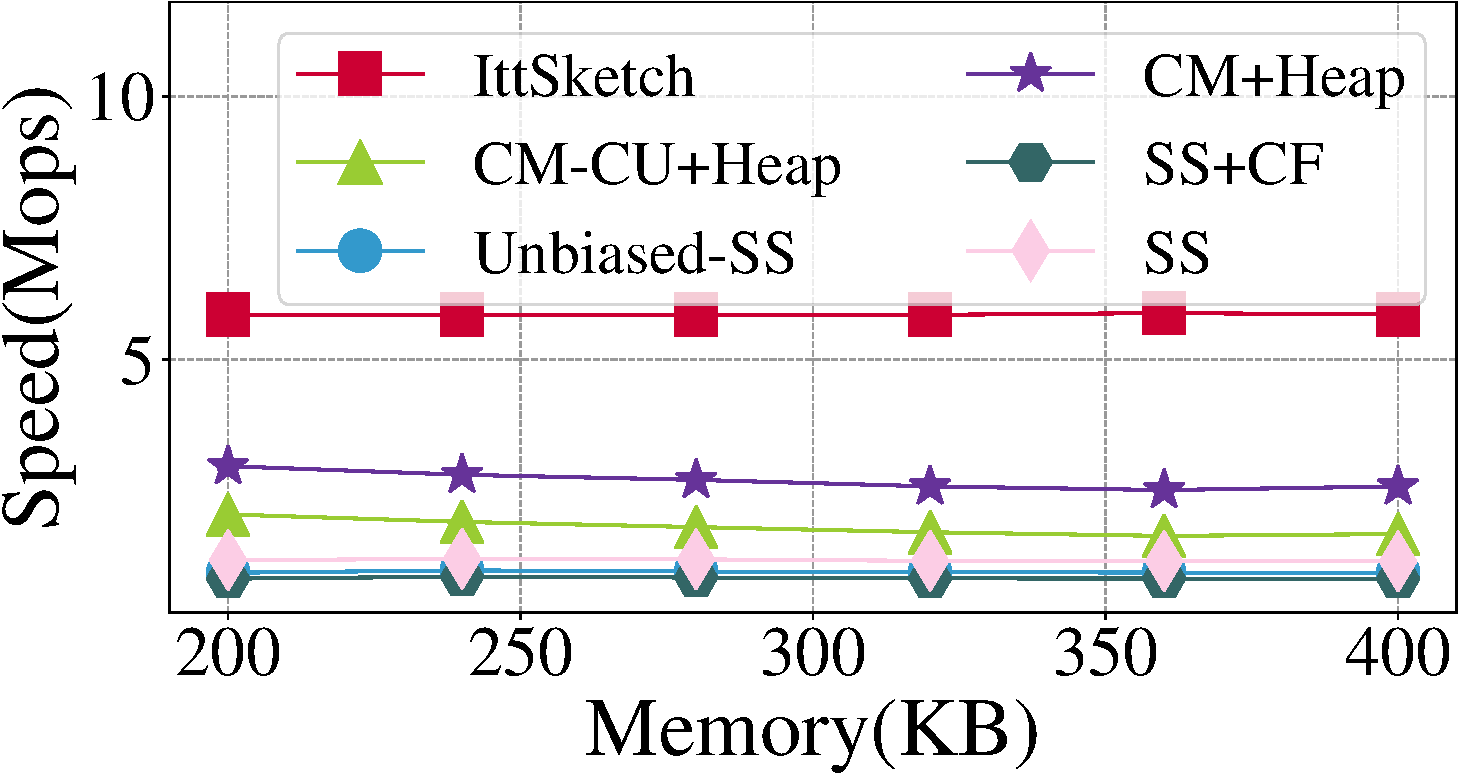
\includegraphics[width=0.95\textwidth, ]{Figures/fre/fre_speed/fre_syn_speed-cropped.pdf}
		\end{center}
		}
		\postfig 
		\adjustfigs
		\prefigcaption
		\label{fre_speed_syn}
		\postfigcaption
		\end{minipage}
	}
	%
	\subfigure[IP trace]{
		\begin{minipage}[t]{0.23\textwidth}{
		\prefig
		\begin{center}
		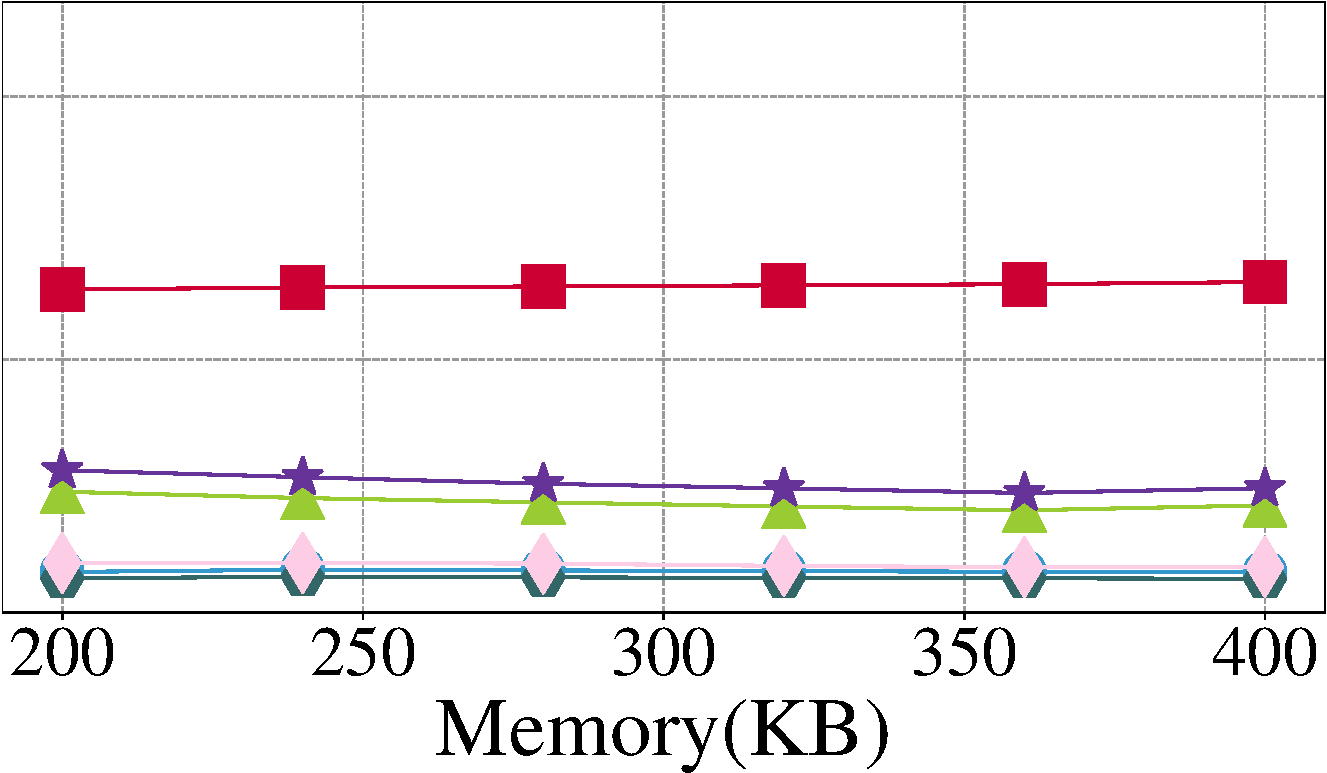
\includegraphics[width=0.95\textwidth, ]{Figures/fre/fre_speed/fre_ip_speed-cropped.pdf}
		\end{center}
		}
		\postfig
		\adjustfigs
		\prefigcaption
		\label{fre_speed_ip}\postfigcaption
		\end{minipage}
	}
	%
	\subfigure[Web page]{
		\begin{minipage}[t]{0.23\textwidth}{
		\prefig
		\begin{center}		
		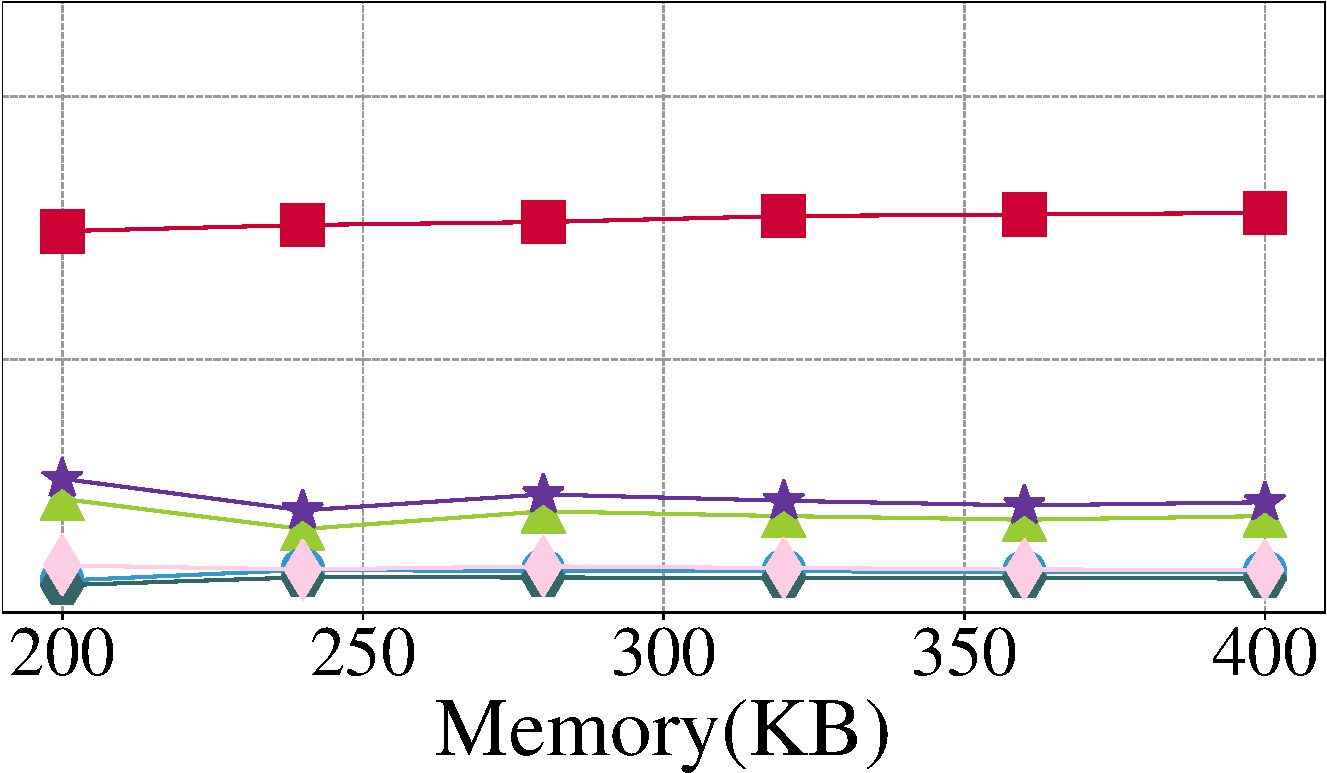
\includegraphics[width=0.95\textwidth, ]{Figures/fre/fre_speed/fre_web_speed-cropped.pdf}
		\end{center}
		}
		\postfig 
		\adjustfigs
		\prefigcaption
		\label{fre_speed_web}
		\postfigcaption
		\end{minipage}
	}
	%
	\subfigure[Network dataset]{
		\begin{minipage}[t]{0.23\textwidth}{
		\prefig
		\begin{center}		
		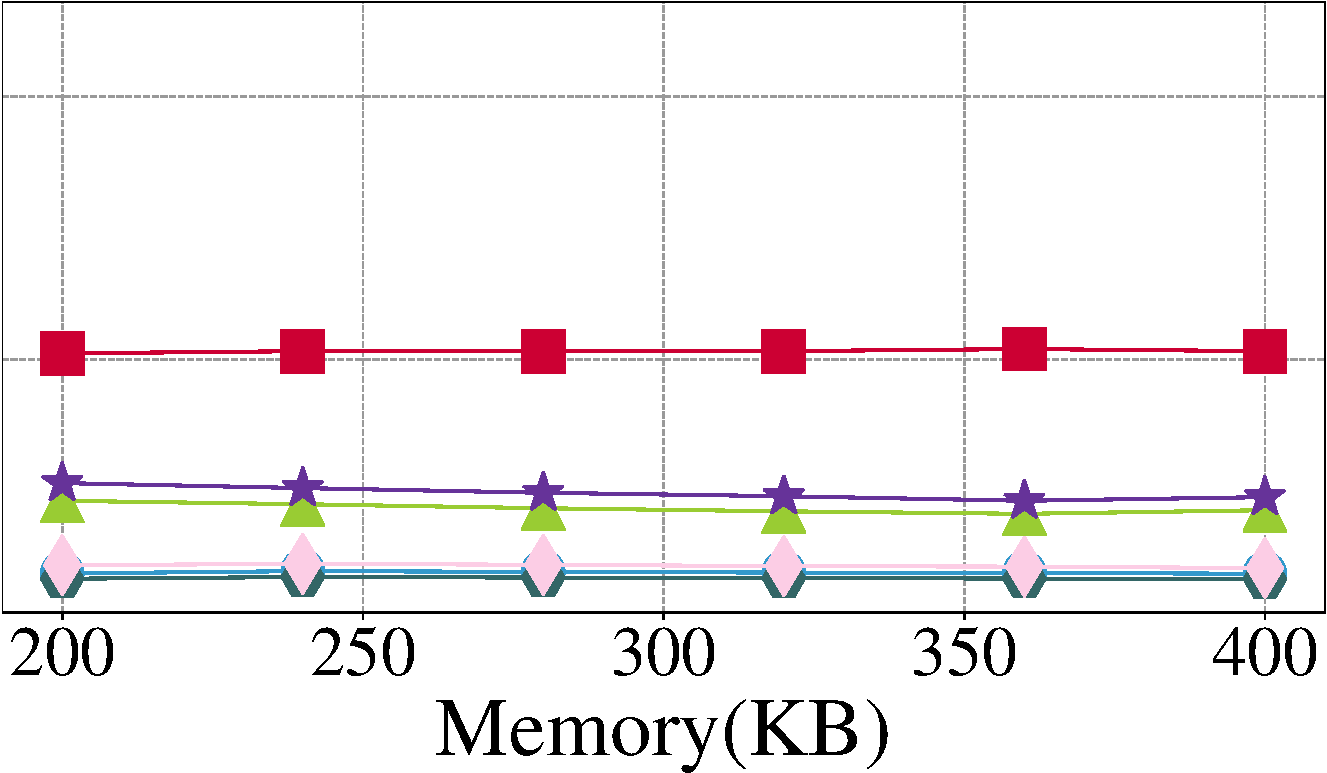
\includegraphics[width=0.95\textwidth, ]{Figures/fre/fre_speed/fre_net_speed-cropped.pdf}
		\end{center}
		}
		\postfig 
		\adjustfigs
		\prefigcaption
		\label{fre_speed_net}
		\postfigcaption
		\end{minipage}
	}
	\vvv \vvv
	\caption{Speed of finding \taskone.}
	\label{fre_speed}
\end{figure*}		
			
\noindent\textbf{Speed (Figure~\ref{fre_speed_syn}-\ref{fre_speed_net}):}
We find that, on three real-world datasets and one synthetic dataset, the insertion speed of \sketchname{} is around 2.2 times, 2.7 times, 7.7 times, 5.48 times, and 6.7 times faster than \freCM, \freCU, \freCF, \freSS{}, and \freunbia{}, respectively.


\noindent\textbf{AAE (Figure~\ref{fre_aae_syn}-\ref{fre_aae_net}) in Appendix \ref{app:fig}:}
We find that, on three real-world datasets, the AAE of \sketchname{} is around 7309 times, 995 times, 3860 times, 3701 times, and 3549 times lower than \freCM, \freCU, \freCF, \freSS{}, and \freunbia{}, respectively. Besides, on the synthetic dataset, the AAE of \sketchname{} is around 2278 times, 80 times, 3247 times, 3278 times, and 3205 times lower than \freCM, \freCU, \freCF, \freSS{}, and \freunbia{}, respectively. 

\begin{figure*}[!ht]
	\centering
	%
	\subfigure[Synthetic dataset]{
		\begin{minipage}[t]{0.255\textwidth}{
		\prefig
		\begin{center}
		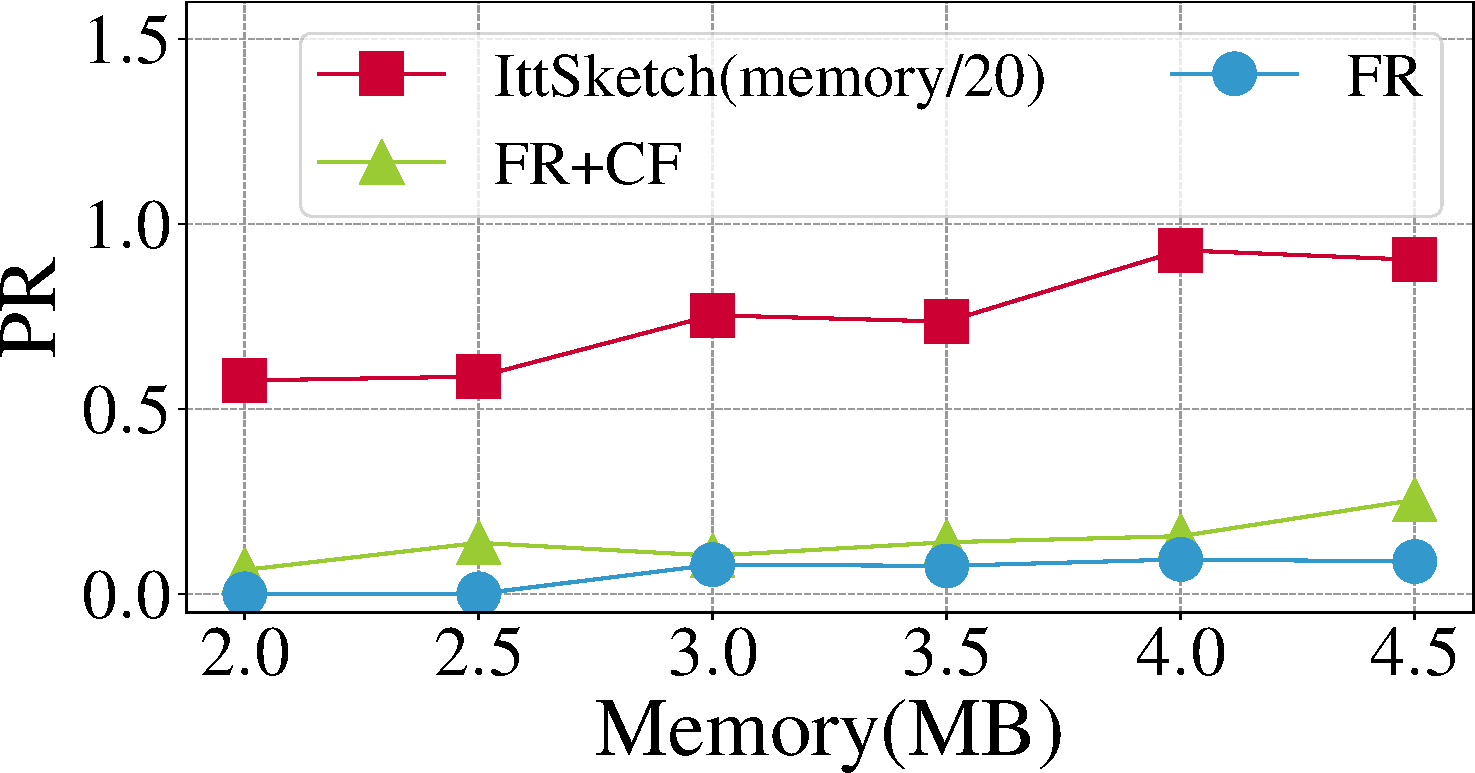
\includegraphics[width=0.95\textwidth, ]{Figures/cha/cha_pr/cha_syn_pr-cropped.pdf}
		\end{center}
		}
		\postfig 
		\adjustfigs
		\prefigcaption
		\label{cha_pr_syn}
		\postfigcaption
		\end{minipage}
	}
	%
	\subfigure[IP trace]{
		\begin{minipage}[t]{0.23\textwidth}{
		\prefig
		\begin{center}
		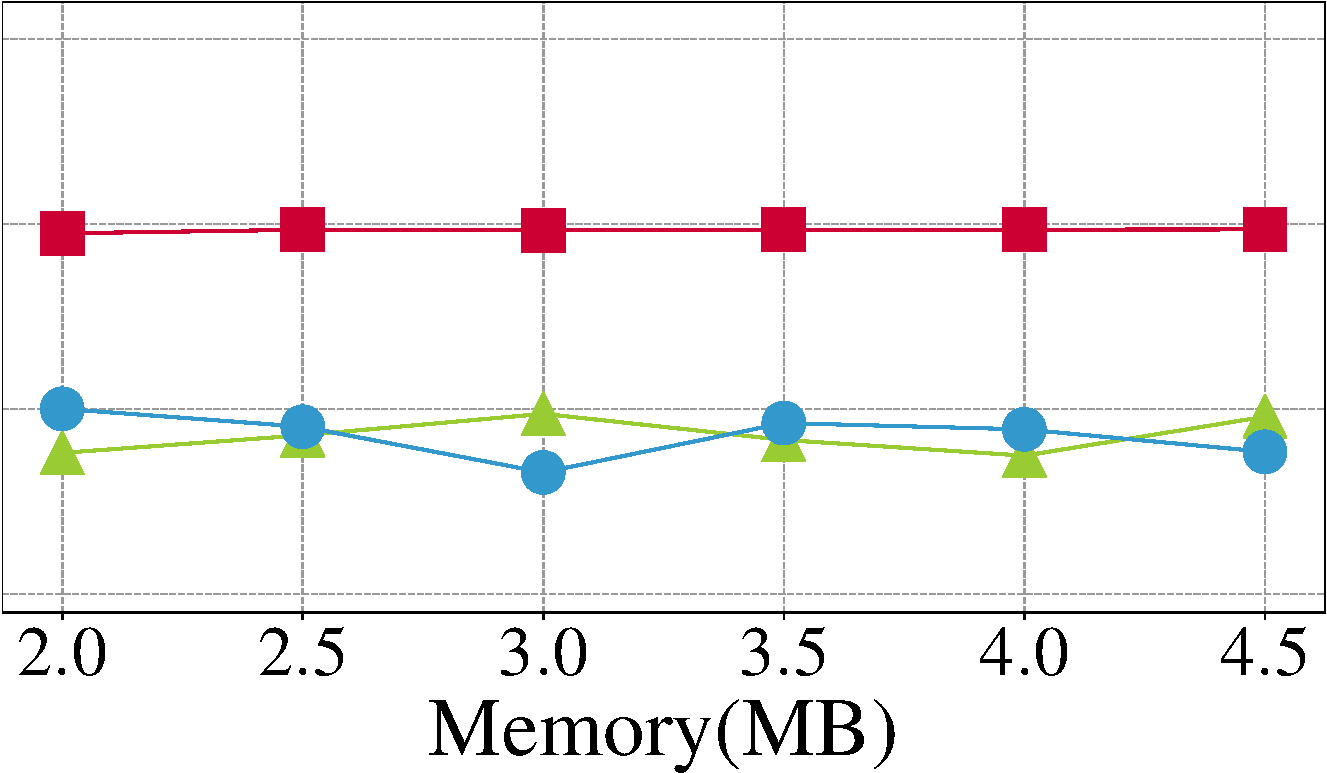
\includegraphics[width=0.95\textwidth, ]{Figures/cha/cha_pr/cha_ip_pr-cropped.pdf}
		\end{center}
		}
		\postfig
		\adjustfigs
		\prefigcaption
		\label{cha_pr_ip}
		\postfigcaption
		\end{minipage}
	}
	%
	\subfigure[Web page]{
		\begin{minipage}[t]{0.23\textwidth}{
		\prefig
		\begin{center}		
		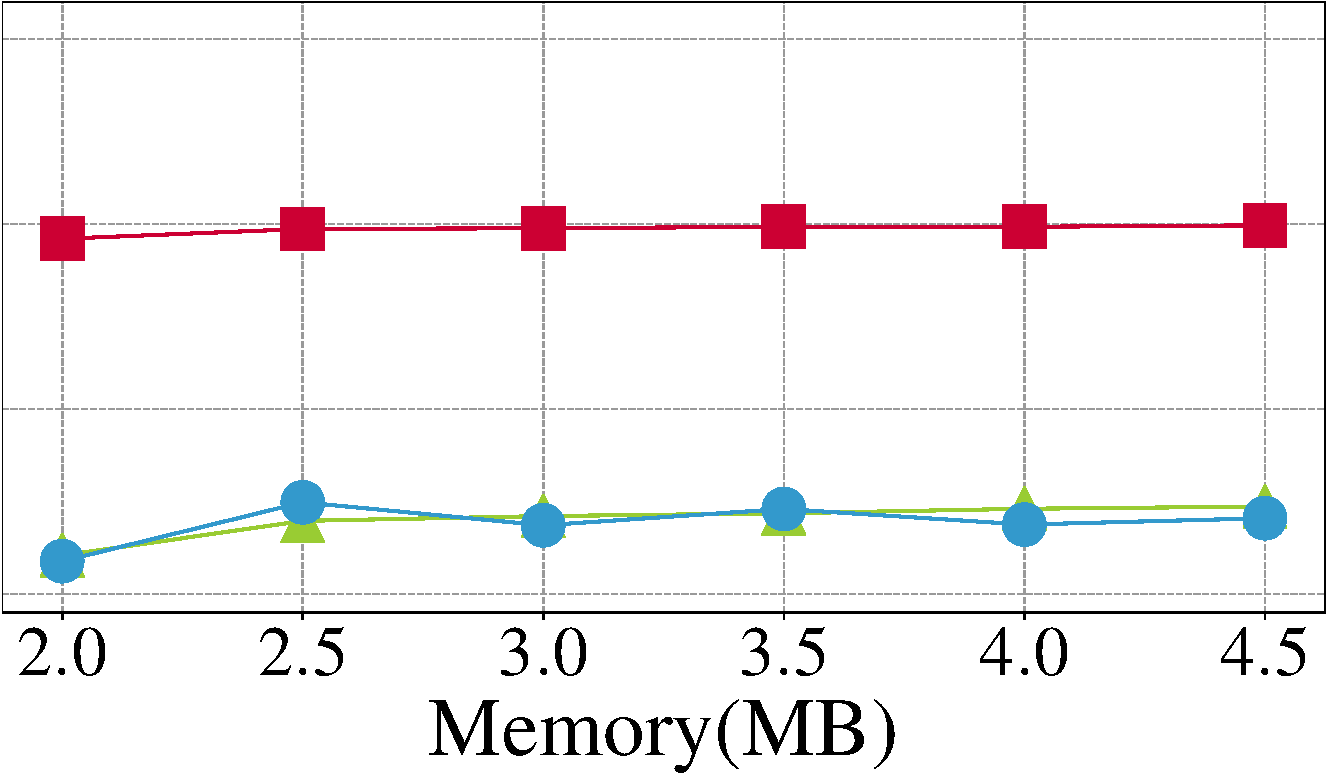
\includegraphics[width=0.95\textwidth, ]{Figures/cha/cha_pr/cha_web_pr-cropped.pdf}
		\end{center}
		}
		\postfig 
		\adjustfigs
		\prefigcaption
		\label{cha_pr_web}
		\postfigcaption
		\end{minipage}
	}
	%
	\subfigure[Network dataset]{
		\begin{minipage}[t]{0.23\textwidth}{
		\prefig
	    \begin{center}		
		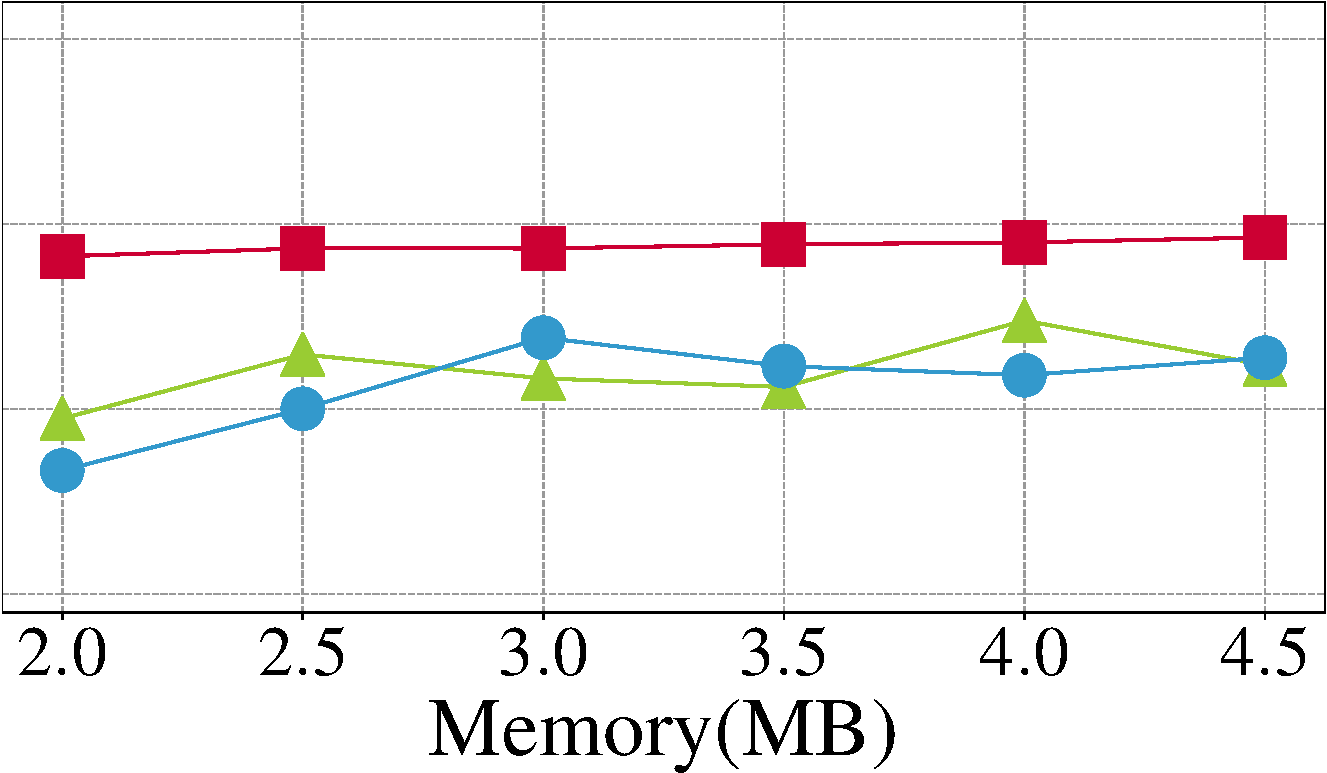
\includegraphics[width=0.95\textwidth, ]{Figures/cha/cha_pr/cha_net_pr-cropped.pdf}
		\end{center}
		}
		\postfig 
		\adjustfigs
		\prefigcaption
		\label{cha_pr_net}
		\postfigcaption
		\end{minipage}
	}
	%
	\vvv \vvv
    \caption{PR of finding \taskfour.}
	\label{cha_pr}
\end{figure*}

\begin{figure*}[!ht]
	\centering
	%
	\subfigure[Synthetic dataset]{
		\begin{minipage}[t]{0.24546\textwidth}{
		\prefig
		\begin{center}
		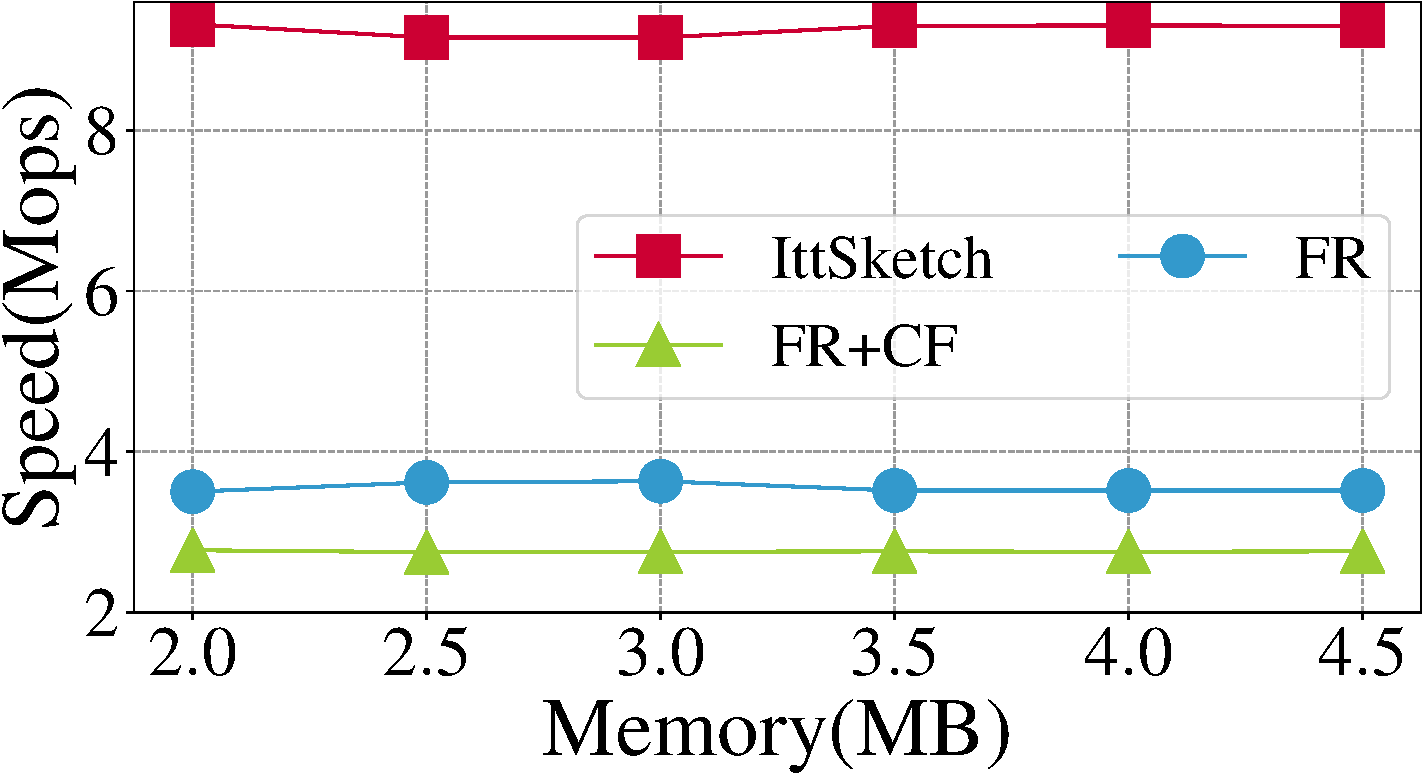
\includegraphics[width=0.95\textwidth, ]{Figures/cha/cha_speed/cha_syn_speed-cropped.pdf}
		\end{center}
		}
		\postfig 
		\adjustfigs
		\prefigcaption
		\label{cha_speed_syn}
		\postfigcaption
		\end{minipage}
	}
	%
	\subfigure[IP trace]{
		\begin{minipage}[t]{0.23\textwidth}{
		\prefig
		\begin{center}
		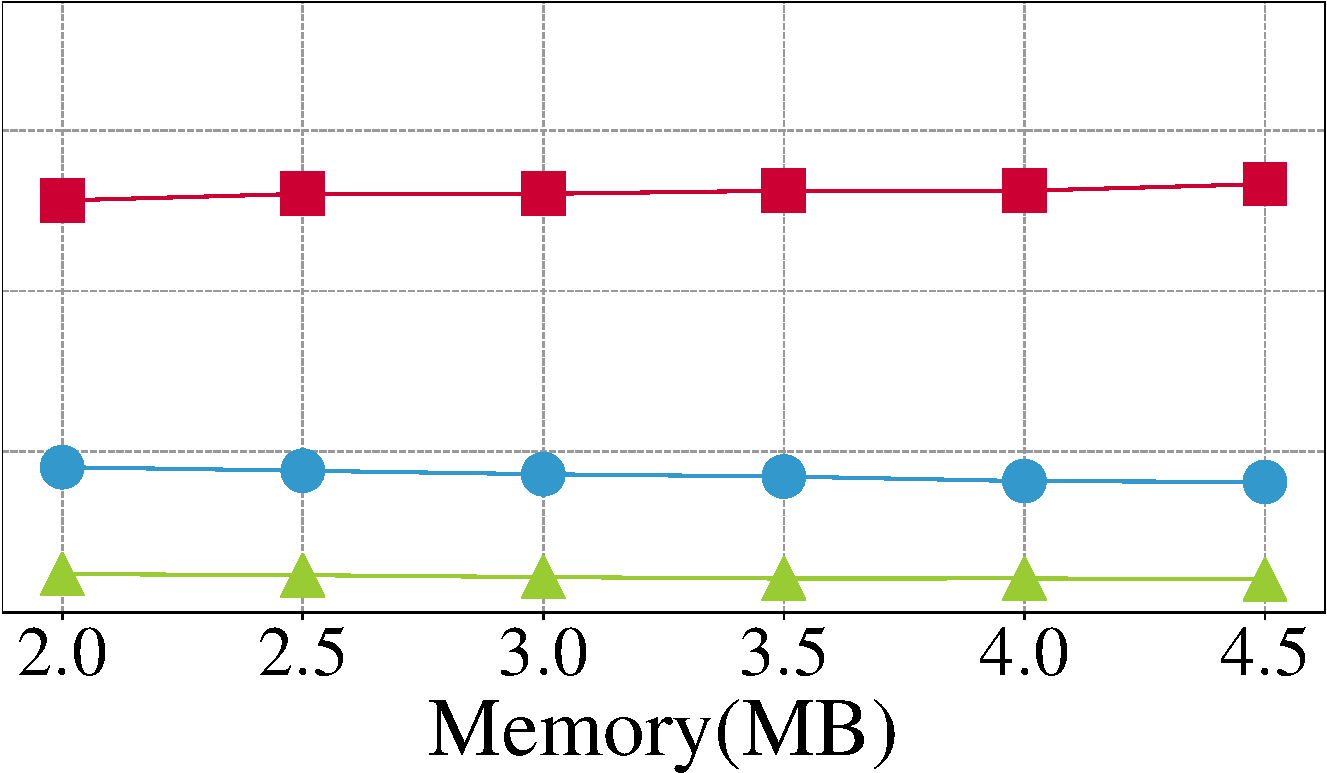
\includegraphics[width=0.95\textwidth, ]{Figures/cha/cha_speed/cha_ip_speed-cropped.pdf}
		\end{center}
		}
		\postfig
		\adjustfigs
		\prefigcaption
		\label{cha_speed_ip}
		\postfigcaption
		\end{minipage}
	}
	%
	\subfigure[Web page]{
		\begin{minipage}[t]{0.23\textwidth}{
		\prefig
		\begin{center}		
		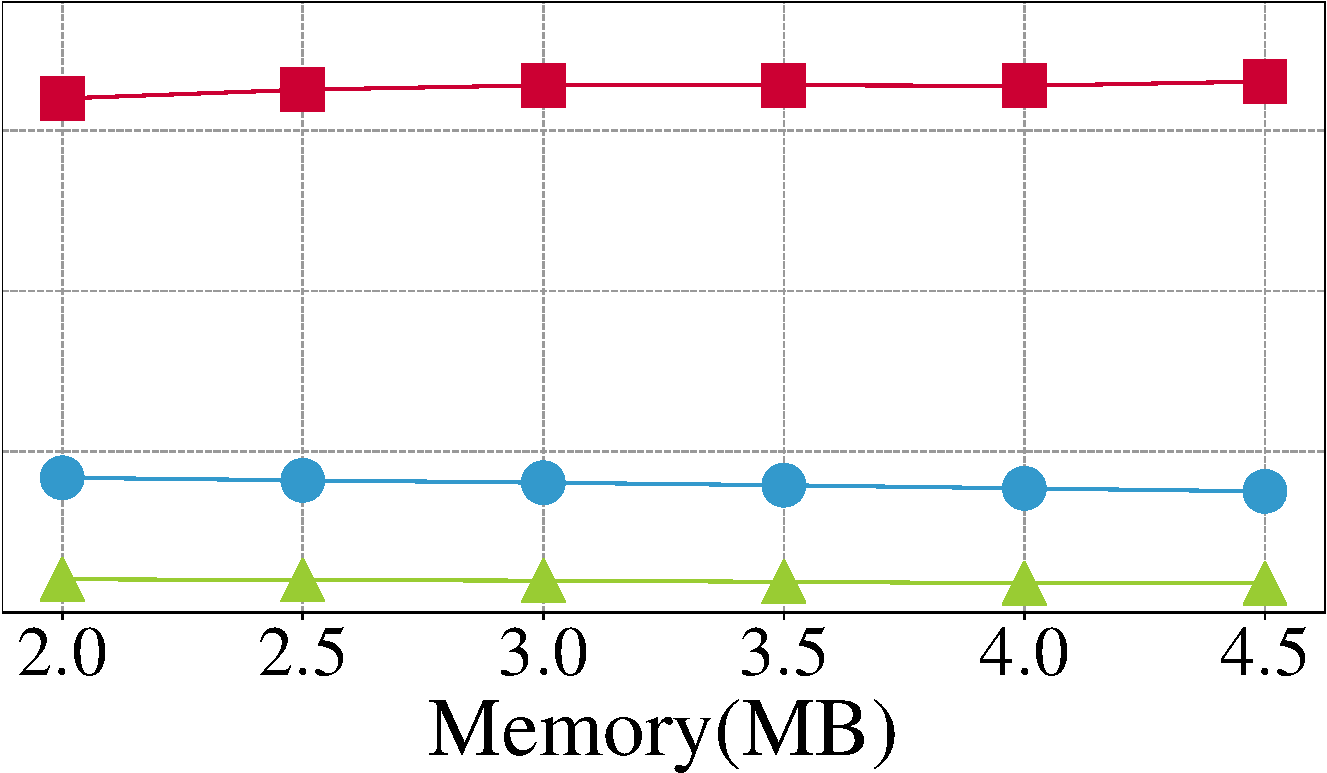
\includegraphics[width=0.95\textwidth, ]{Figures/cha/cha_speed/cha_web_speed-cropped.pdf}
		\end{center}
		}
		\postfig 
		\adjustfigs
		\prefigcaption
		\label{cha_speed_web}
		\postfigcaption
		\end{minipage}
	}
	%
	\subfigure[Network dataset]{
		\begin{minipage}[t]{0.23\textwidth}{
		\prefig
		\begin{center}		
		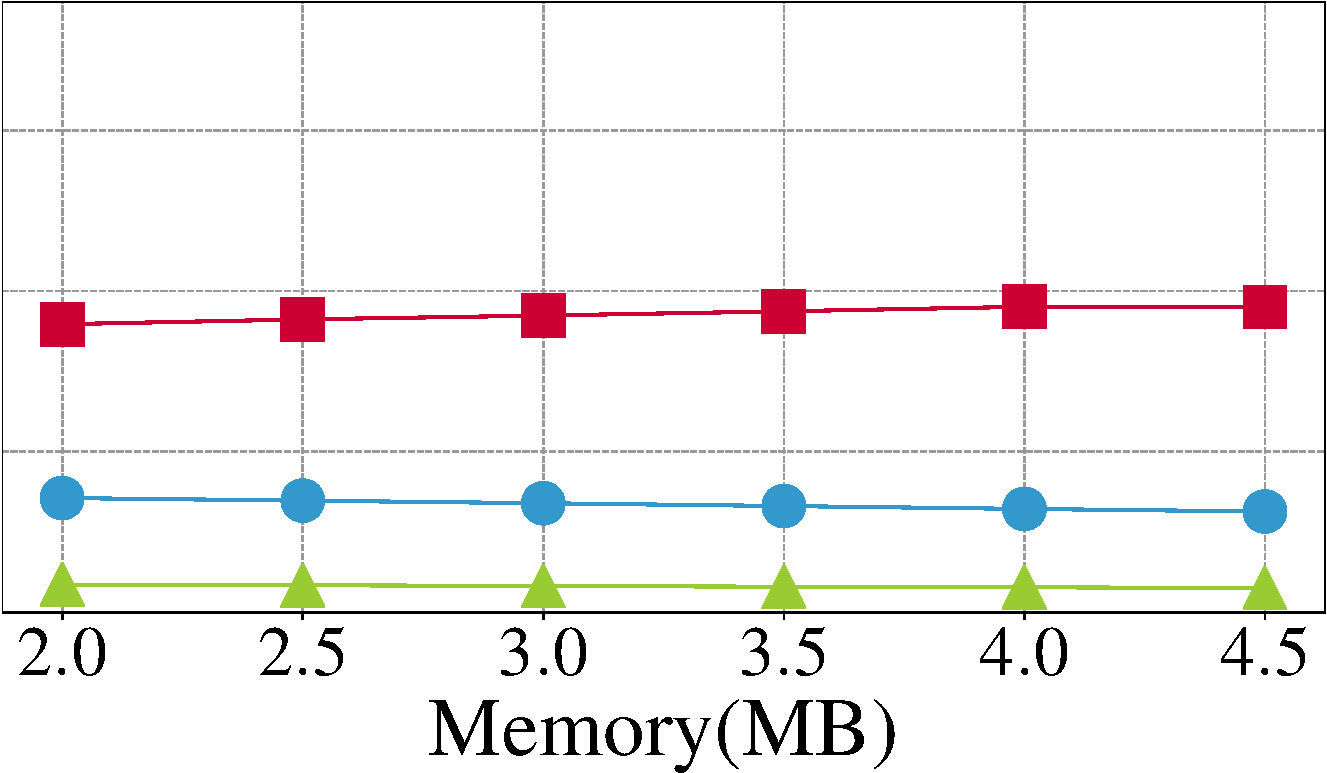
\includegraphics[width=0.95\textwidth, ]{Figures/cha/cha_speed/cha_net_speed-cropped.pdf}
		\end{center}
		}
		\postfig 
		\adjustfigs
		\prefigcaption
		\label{cha_speed_net}
		\postfigcaption
		\end{minipage}
	}
	%
	\vvv \vvv
    \caption{Speed of finding \taskfour.}
	\label{cha_speed}
\end{figure*}

\noindent\textbf{CR (Figure~\ref{fre_cr_syn}-\ref{fre_cr_net}) in Appendix \ref{app:fig}:}
We find that, on three real-world datasets, the CR of \sketchname{} is around 5.6 times, 5 times, 1.7 times, 2 times, and 1.6 times higher than \freCM, \freCU, \freCF, \freSS{}, and \freunbia{}, respectively. 
On the synthetic dataset, the CR of \sketchname{} is around 17 times, 18 times, 5 times, 4.7 times, and 5.3 times higher than \freCM, \freCU, \freCF, \freSS{}, and \freunbia{}, respectively.


\noindent\textbf{Summary:}
%
1) \sketchname{} can achieve high accuracy with limited memory. The ARE of \sketchname{} is lower than 0.01 when the memory is set to 200KB, while the ARE of the other algorithms is often higher than 1. As seen in the figures, the ARE of \freSS, \freCF{}, and \freunbia{} often exceed the range of the plots.

2) \sketchname{} can report more correct instances than other approaches. \sketchname{} often reports more than 99 percent of the correct instances, while the other approaches report less than 40 percent, because they often consume too much memory on the hash table or Stream-Summary.

3) \sketchname{} achieves higher precision in reported instances. The PR of \sketchname{} is often higher than 0.99, while the PR of other approaches is often less than 0.6 because they overestimate the results. 

4) The insertion speed of \sketchname{} is also faster than the other approaches for the same memory consumption on three real-world datasets and one synthetic dataset.
\begin{figure*}[!ht]
	\centering
	%
	\subfigure[IP trace1]{
		\begin{minipage}[t]{0.255\textwidth}{
		\prefig
		\begin{center}
		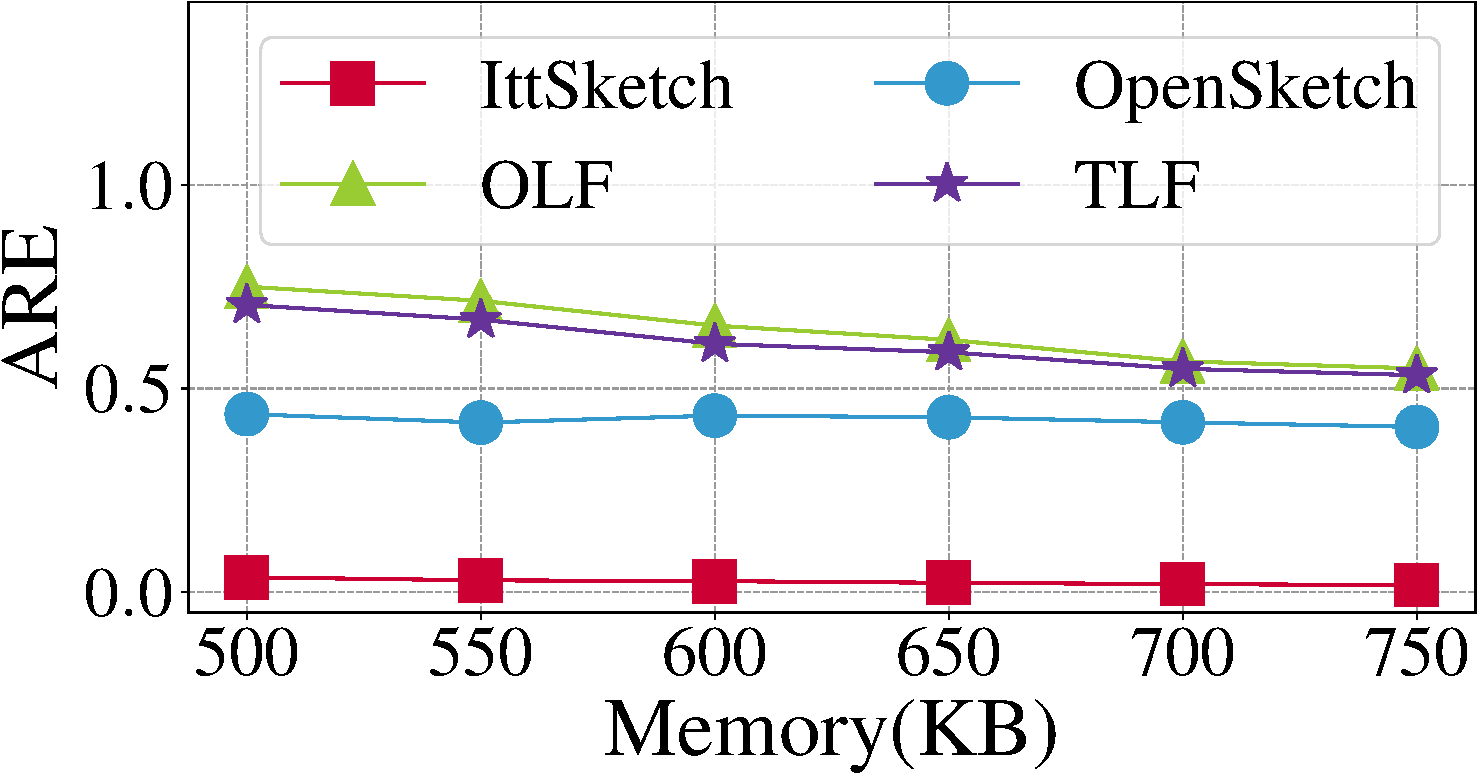
\includegraphics[width=0.95\textwidth, ]{Figures/sup/sup_are/_sup_ip_are.pdf}
		\end{center}
		}
		\postfig
		\adjustfigs
		\prefigcaption
		\label{sup_are_ip}
		\postfigcaption
		\end{minipage}
	}
	%
	\subfigure[IP trace2]{
		\begin{minipage}[t]{0.23\textwidth}{
		\prefig
		\begin{center}		
		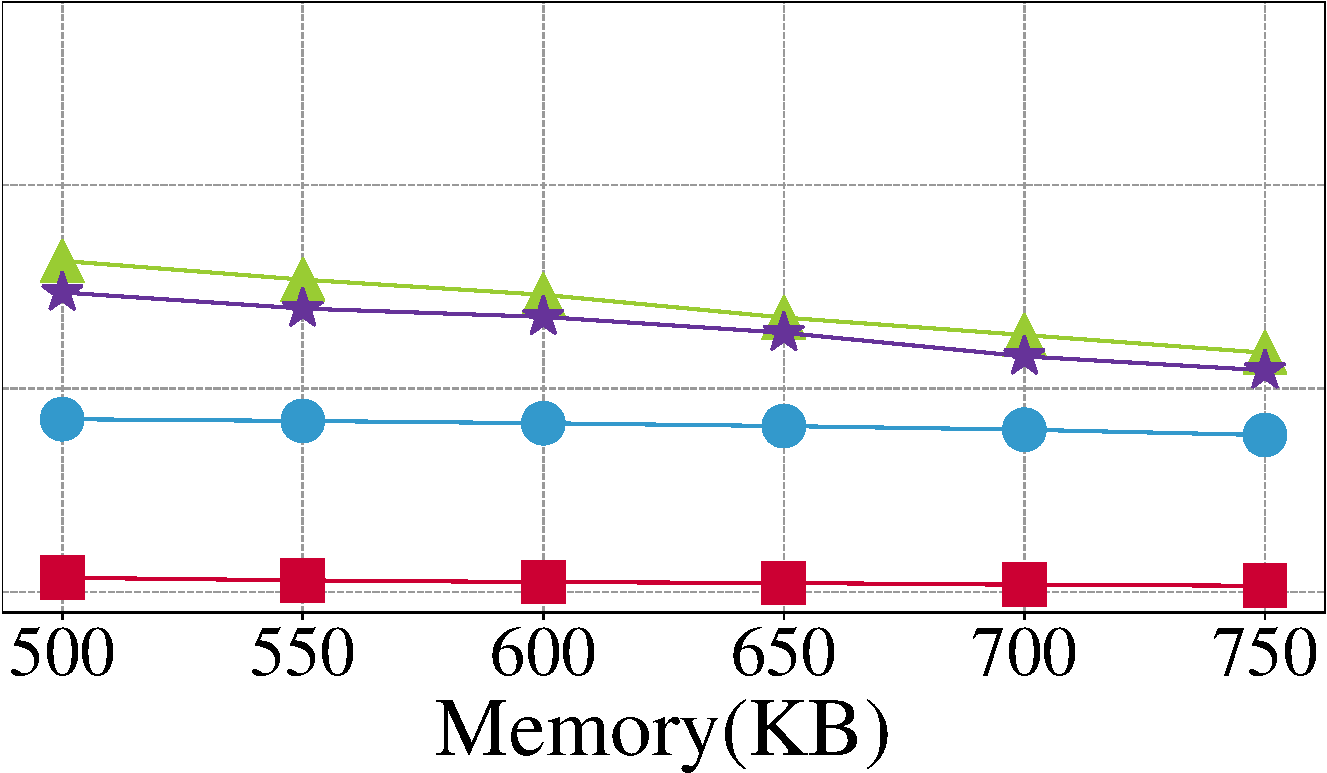
\includegraphics[width=0.95\textwidth, ]{Figures/sup/sup_are/_sup_ip4_are.pdf}
		\end{center}
		}
		\postfig 
		\adjustfigs
		\prefigcaption
		\label{sup_are_ip4}
		\postfigcaption
		\end{minipage}
	}
	%
	\subfigure[IP trace3]{
		\begin{minipage}[t]{0.23\textwidth}{
		\prefig
		\begin{center}		
		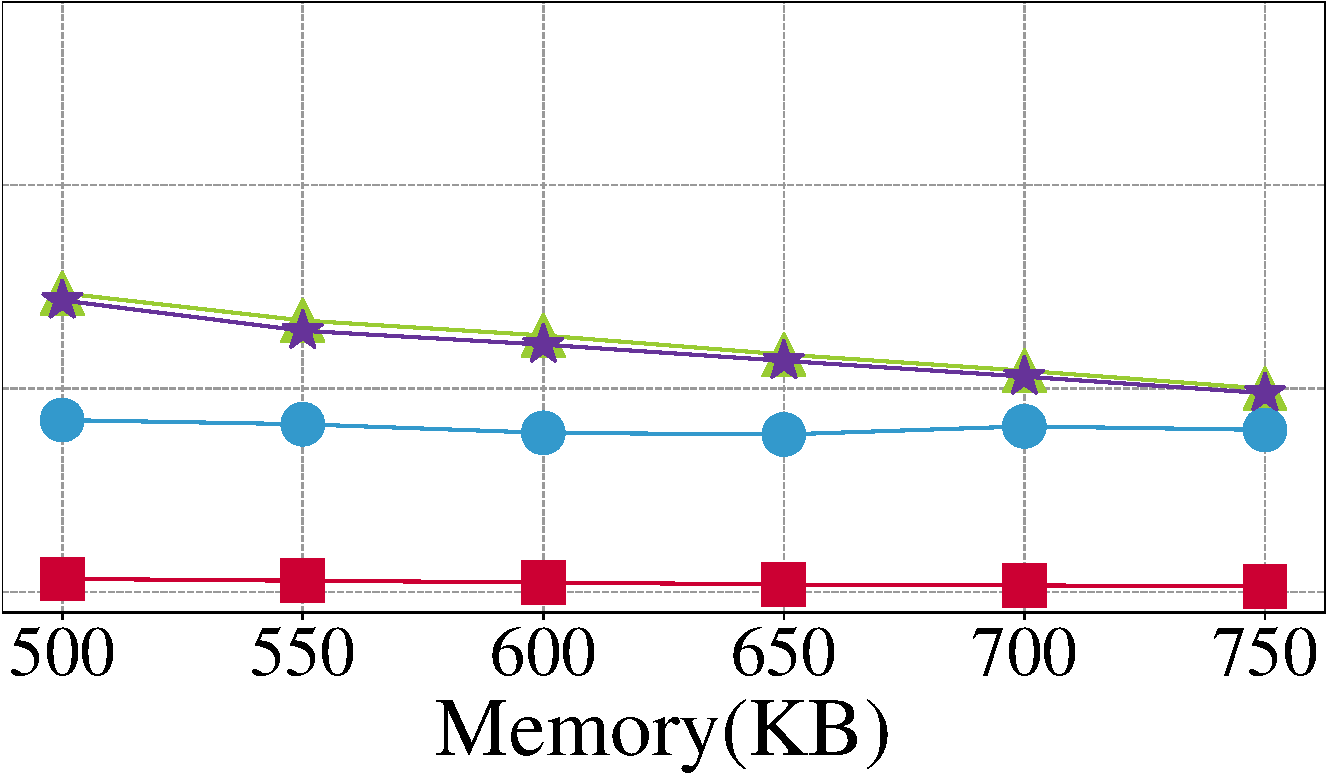
\includegraphics[width=0.95\textwidth, ]{Figures/sup/sup_are/_sup_ip6_are.pdf}
		\end{center}
		}
		\postfig 
		\adjustfigs
		\prefigcaption
		\label{sup_are_ip6}
		\postfigcaption
		\end{minipage}
	}
	%
	\subfigure[IP trace4]{
	    \begin{minipage}[t]{0.23\textwidth}{
		\prefig
		\begin{center}
		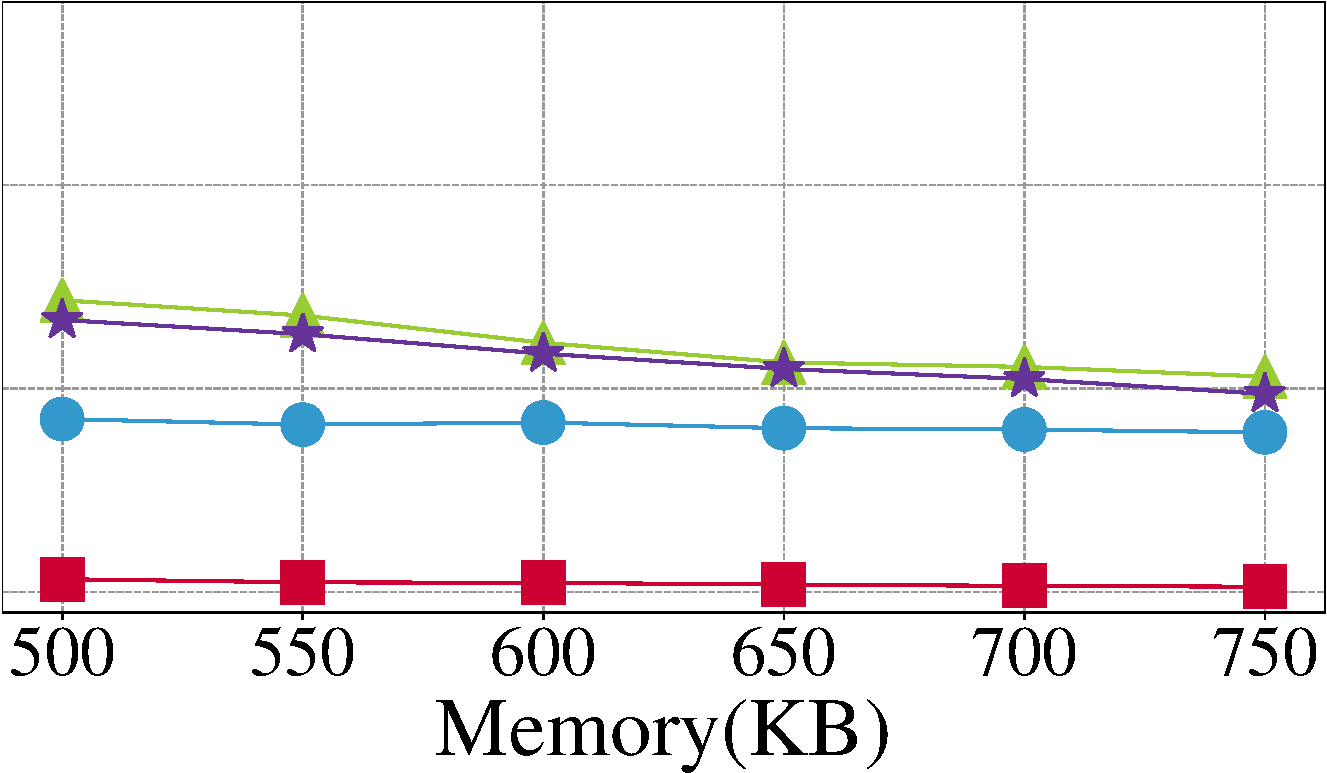
\includegraphics[width=0.95\textwidth, ]{Figures/sup/sup_are/_sup_ip8_are.pdf}
		\end{center}
		}
		\postfig 
		\adjustfigs
		\prefigcaption
		\label{sup_are_ip8}
		\postfigcaption
		\end{minipage}
	}
	%
	\vvv \vvv
    \caption{ARE of finding \tasktwo.}
	\label{sup_are}
\end{figure*}


\begin{figure*}[!ht]
	\centering
	%
	\subfigure[IP trace1]{
		\begin{minipage}[t]{0.255\textwidth}{
		\prefig
		\begin{center}
		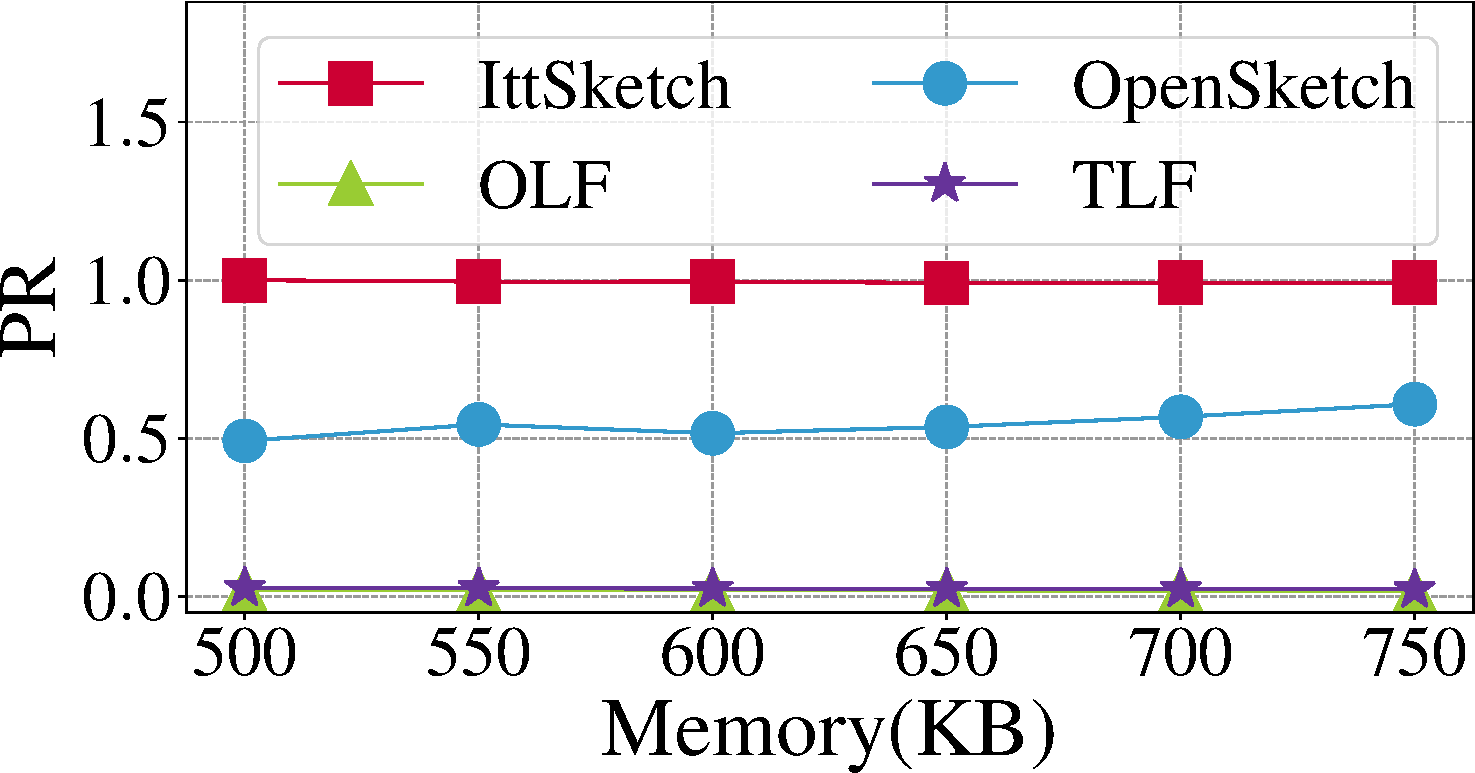
\includegraphics[width=0.95\textwidth, ]{Figures/sup/sup_pr/_sup_ip_pr.pdf}
		\end{center}
		}
		\postfig
		\adjustfigs
		\prefigcaption
		\label{sup_pr_ip}
		\postfigcaption
		\end{minipage}
	}
	%
	\subfigure[IP trace2]{
		\begin{minipage}[t]{0.23\textwidth}{
		\prefig
		\begin{center}		
		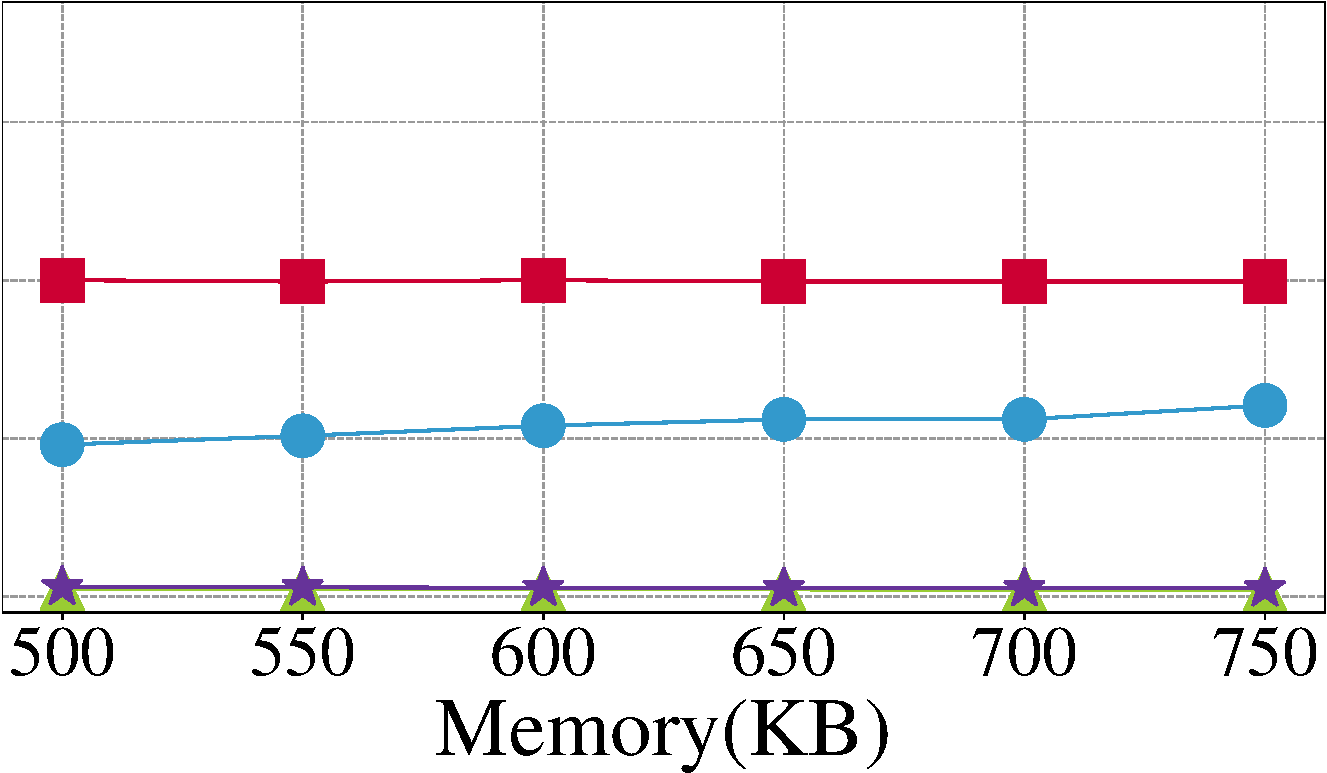
\includegraphics[width=0.95\textwidth, ]{Figures/sup/sup_pr/_sup_ip4_pr.pdf}
		\end{center}
		}
		\postfig 
		\adjustfigs
		\prefigcaption
		\label{sup_pr_ip4}
		\postfigcaption
		\end{minipage}
	}
	%
	\subfigure[IP trace3]{
		\begin{minipage}[t]{0.23\textwidth}{
		\prefig
		\begin{center}		
		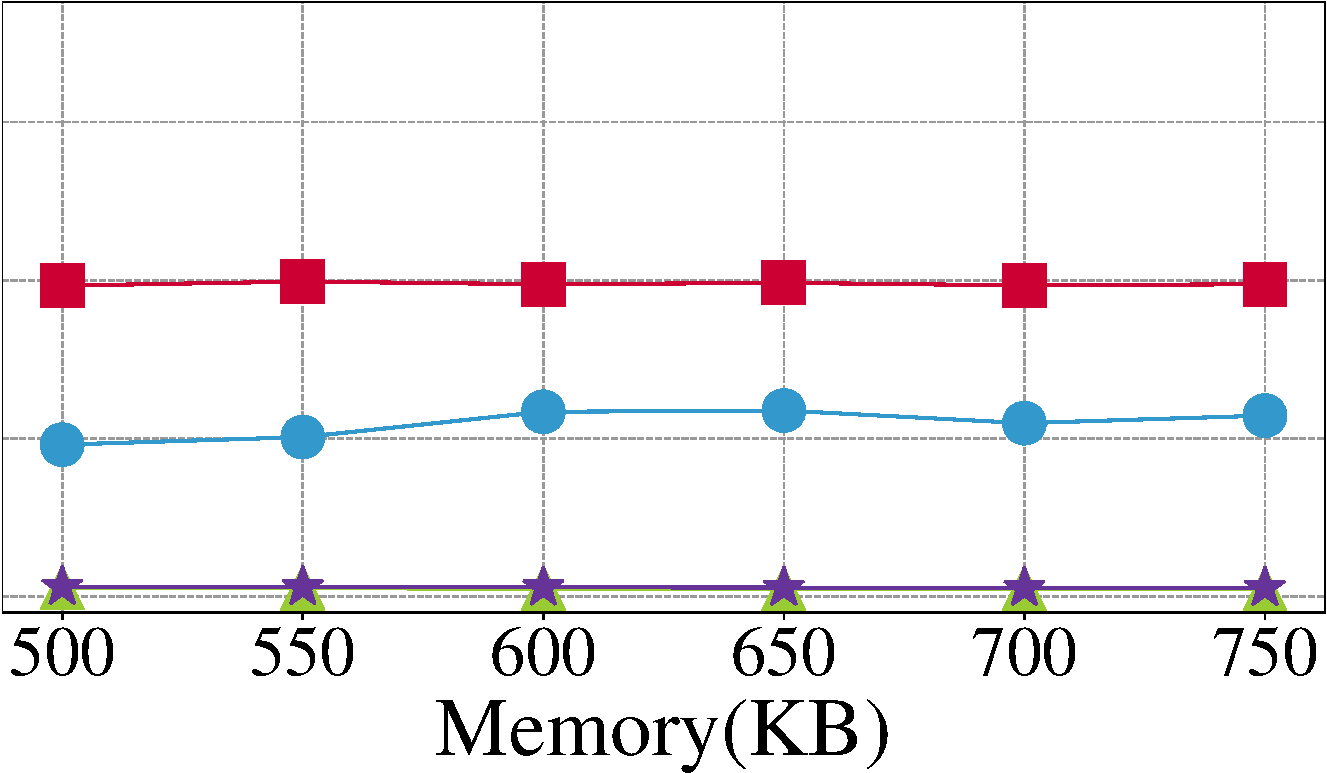
\includegraphics[width=0.95\textwidth, ]{Figures/sup/sup_pr/_sup_ip6_pr.pdf}
		\end{center}
		}
		\postfig 
		\adjustfigs
		\prefigcaption
		\label{sup_pr_ip6}
		\postfigcaption
		\end{minipage}
	}
	%
	\subfigure[IP trace4]{
		\begin{minipage}[t]{0.23\textwidth}{
		\prefig
		\begin{center}
		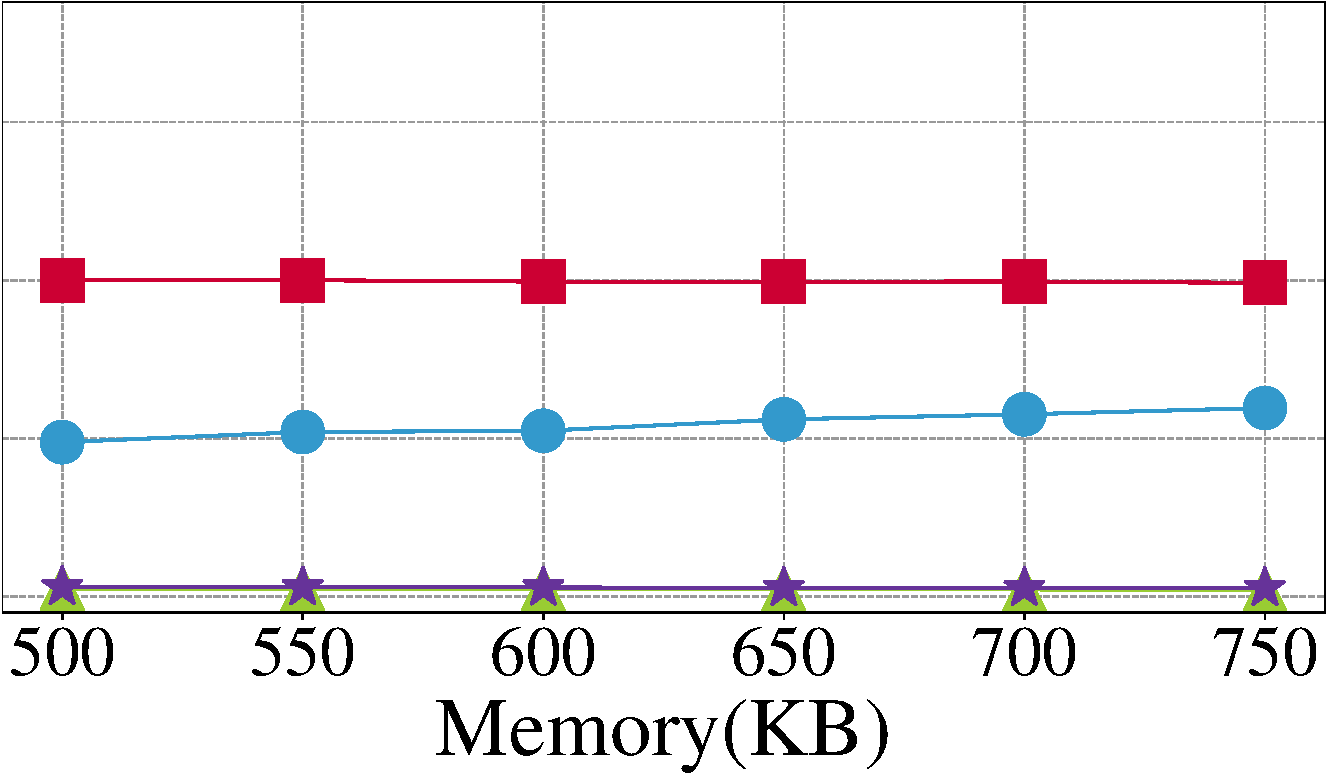
\includegraphics[width=0.95\textwidth, ]{Figures/sup/sup_pr/_sup_ip8_pr.pdf}
		\end{center}
		}
		\postfig 
		\adjustfigs
		\prefigcaption
		\label{sup_pr_ip8}
		\postfigcaption
		\end{minipage}
	}
	%
	\vvv \vvv
    \caption{PR of finding \tasktwo.}
	\label{sup_pr}
\end{figure*}

\begin{figure*}[!ht]
	\centering
	%
	\subfigure[IP trace1]{
		\begin{minipage}[t]{0.247\textwidth}{
		\prefig
		\begin{center}
		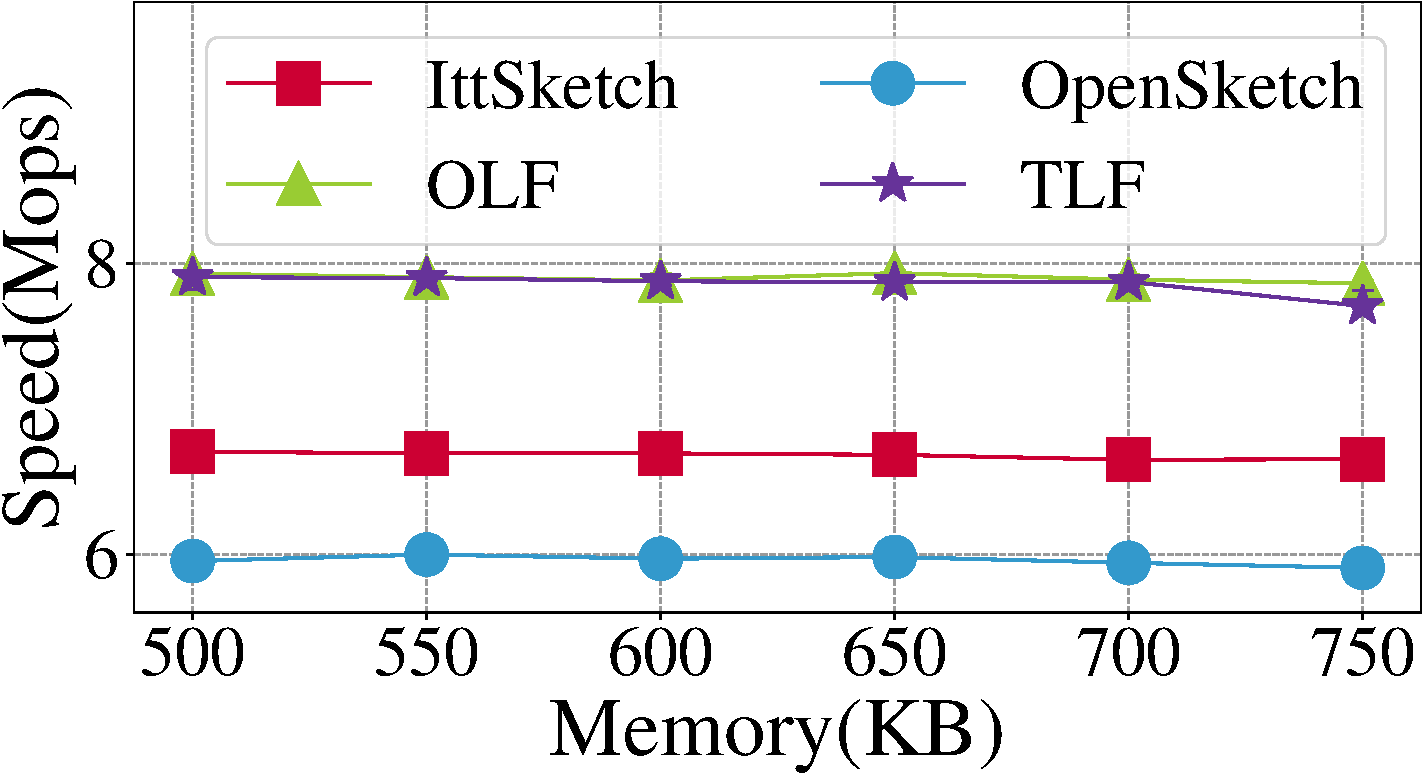
\includegraphics[width=0.95\textwidth, ]{Figures/sup/sup_speed/_sup_ip_speed.pdf}
	    \end{center}
	    }
		\postfig
		\adjustfigs
		\prefigcaption
		\label{sup_speed_ip}
		\postfigcaption
		\end{minipage}
	}
	%
	\subfigure[IP trace2]{
		\begin{minipage}[t]{0.23\textwidth}{				\prefig
		\begin{center}		
		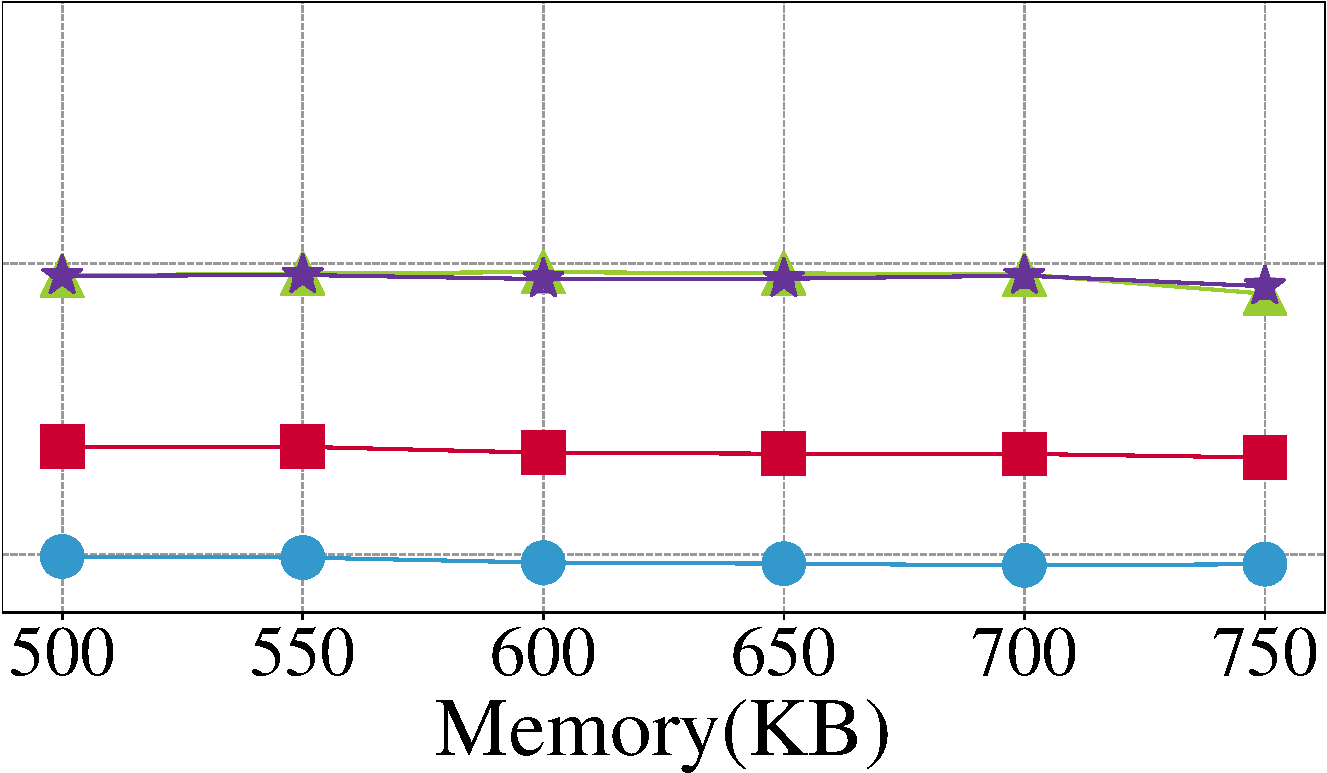
\includegraphics[width=0.95\textwidth, ]{Figures/sup/sup_speed/_sup_ip4_speed.pdf}
		\end{center}
		}
		\postfig 
		\adjustfigs
		\prefigcaption
		\label{sup_speed_ip4}
		\postfigcaption
		\end{minipage}
	}
	%
	\subfigure[IP trace3]{
		\begin{minipage}[t]{0.23\textwidth}{
		\prefig
		\begin{center}		
		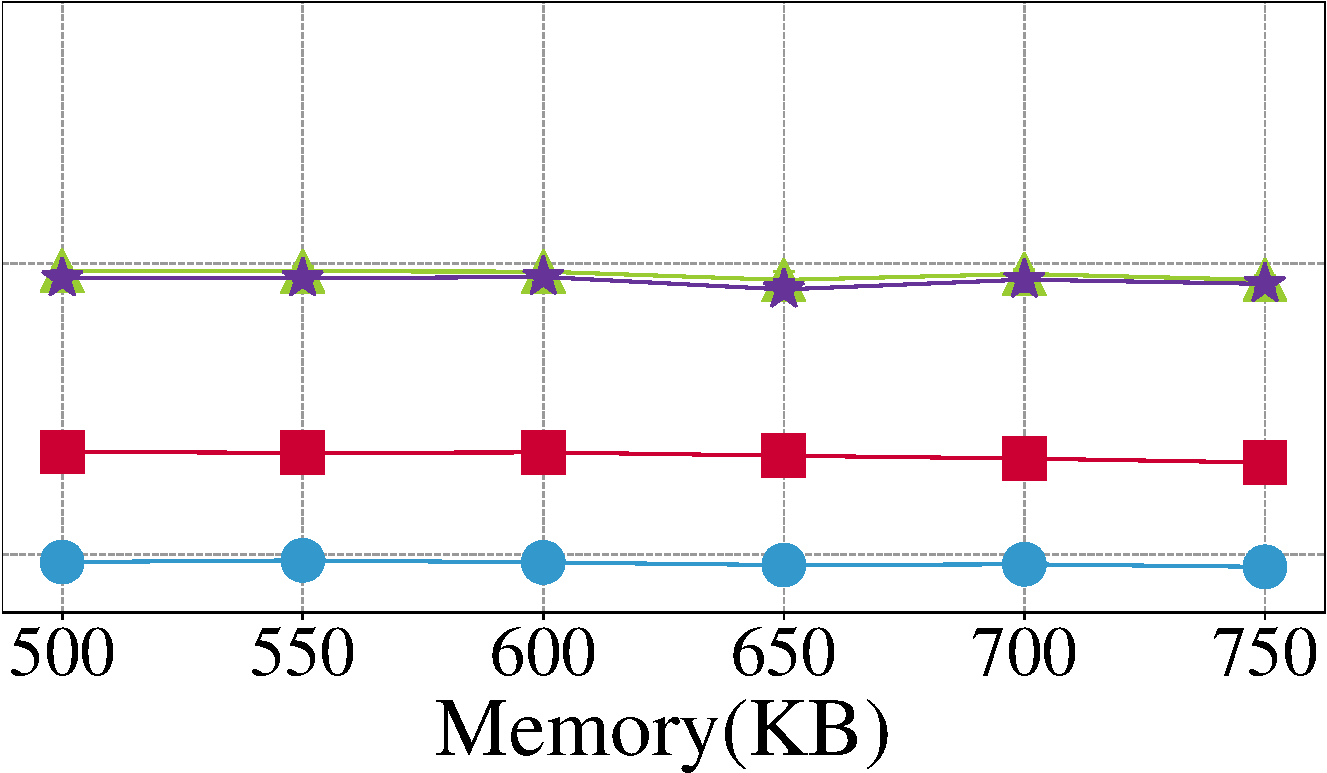
\includegraphics[width=0.95\textwidth, ]{Figures/sup/sup_speed/_sup_ip6_speed.pdf}
		\end{center}
		}
		\postfig 
		\adjustfigs
		\prefigcaption
		\label{sup_speed_ip6}
		\postfigcaption
		\end{minipage}
	}
	%
	\subfigure[IP trace4]{
		\begin{minipage}[t]{0.23\textwidth}{
		\prefig
		\begin{center}
		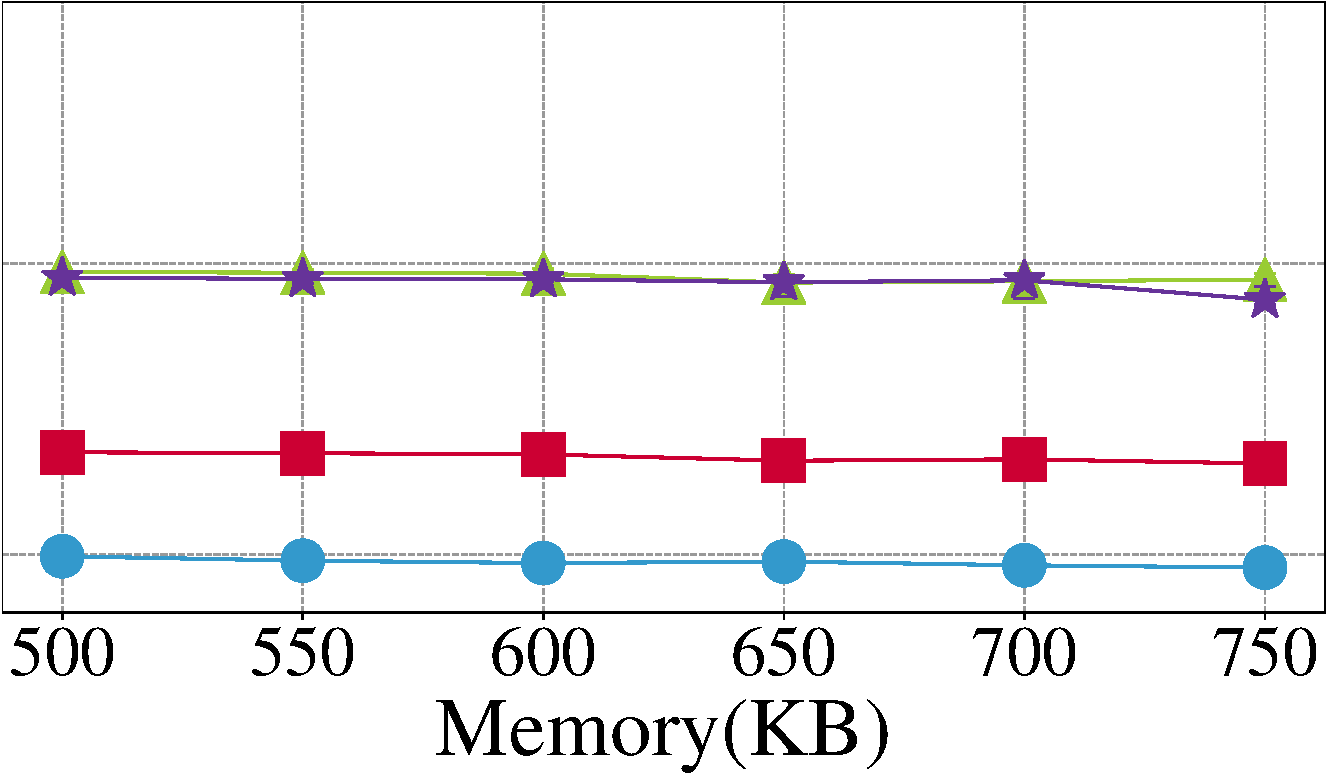
\includegraphics[width=0.95\textwidth, ]{Figures/sup/sup_speed/_sup_ip8_speed.pdf}
		\end{center}
		}
		\postfig 
		\adjustfigs
		\prefigcaption
		\label{sup_speed_ip8}
		\postfigcaption
		\end{minipage}
	}
	%
	\vvv \vvv
    \caption{Speed of finding \tasktwo.}
	\label{sup_speed}
\end{figure*}

%\presub
\subsection{Evaluation on Finding \taskfour} %\postsub
\label{eva_four}

\noindent\textbf{Parameter Setting:}
%We compare three frameworks: \sketchname, \EHname and \Splittername. For each frameworks, we using CM Sketch, CM-CU Sketch and Count Sketch approaches.
%
%We compare 5 approaches: CM \sketchname, CM-CU \sketchname, Count \sketchname, \EHname {} and \Splittername.
We compare 3 algorithms: \sketchname, \chafr\cite{flowradar}, and \chafrcf\cite{coldfilter}.
For \chafr{} and \chafrcf, the parameters are set according to the recommendation of the authors.
In the experiments, we compare PR, CR, and the insertion speed among the 3 algorithms. We vary the amount of memory from from 2MB to 4.5MB. We choose this range because \chafr{} cannot report any heavy changes if memory size is smaller. Also, we set the memory size of \sketchname{} to $1/20$ of the memory size of the other algorithms when we compare PR and CR. The reason for this is that when memory is larger than 2MB, the CR and PR of \sketchname{} are 1. 
%To compare these algorithms more conveniently, we reduce the memory size of \sketchname.


\noindent\textbf{PR (Figure~\ref{cha_pr_syn}-\ref{cha_pr_net}):}
We find that on three real-world datasets, the PR of \sketchname{} is around 4.1 times and 3.6 times higher than \chafr{} and \chafrcf. 
On the synthetic dataset, the PR of \chafr{} is 0 when its memory size is less than 2.5 MB. The PR of \sketchname{} is around 6.2 times higher than \chafrcf. 
			
			
\noindent\textbf{Speed (Figure~\ref{cha_speed_syn}-\ref{cha_speed_net}):}
We find that the insertion speed of \sketchname{} is around 2.1 times and 3 times faster than \chafr{} and \chafrcf{} on three real-world datasets and one synthetic dataset.

\noindent\textbf{CR (Figure~\ref{cha_cr_syn}-\ref{cha_cr_net}) in Appendix \ref{app:fig}:}
We find that, on three real-world datasets, the CR of \sketchname{} is around 64 times and 35 times higher than \chafr{} and \chafrcf. 
On the synthetic dataset, the CR of \chafr{} is 0 when its memory size is less than 2.5 MB. The CR of \sketchname{} is around 16 times higher than \chafrcf. 


\noindent\textbf{Summary:}
%
1) Although the memory size of \sketchname{} is only $1/20$ of other algorithms, the CR of \sketchname{} is often more than 0.98 when its memory size is more than 0.98 on three real-world datasets and one synthetic dataset. 
% Steve: broken sentence, please fix it.
In contrast, the CR of \chafr{} is often lower than 0.2 because it will decode few items if the memory size is too small.

2) The PR of \sketchname{} is lower than the PR of \sketchname~ in other datasets, for there are less differences between the two periods in the synthetic dataset. Therefore, we have to spend more space on finding heavy changes in the synthetic dataset. However, \sketchname{} still performs much better than \chafr{} and \chafrcf.
\begin{figure*}[!ht]
	\centering
	%
	\subfigure[Synthetic dataset]{
		\begin{minipage}[t]{0.2543\textwidth}{
		\prefig
		\begin{center}
		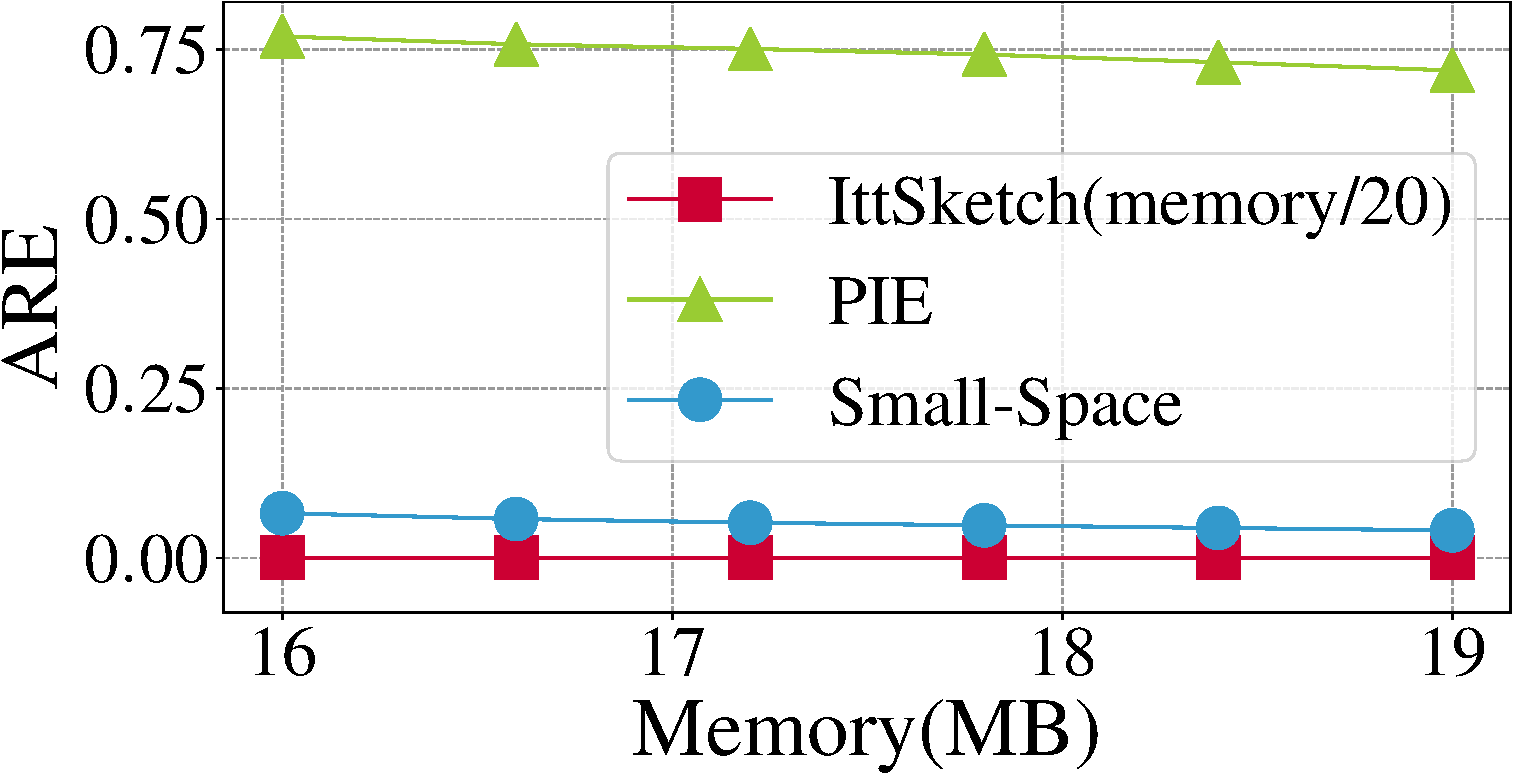
\includegraphics[width=0.95\textwidth, ]{Figures/per/per_are/per_syn_are-cropped.pdf}
		\end{center}
		}
		\postfig 
		\adjustfigs
		\prefigcaption
		\label{per_are_syn}
		\postfigcaption
		\end{minipage}
	}
	%
	\subfigure[IP trace]{
		\begin{minipage}[t]{0.225\textwidth}{
		\prefig
		\begin{center}
		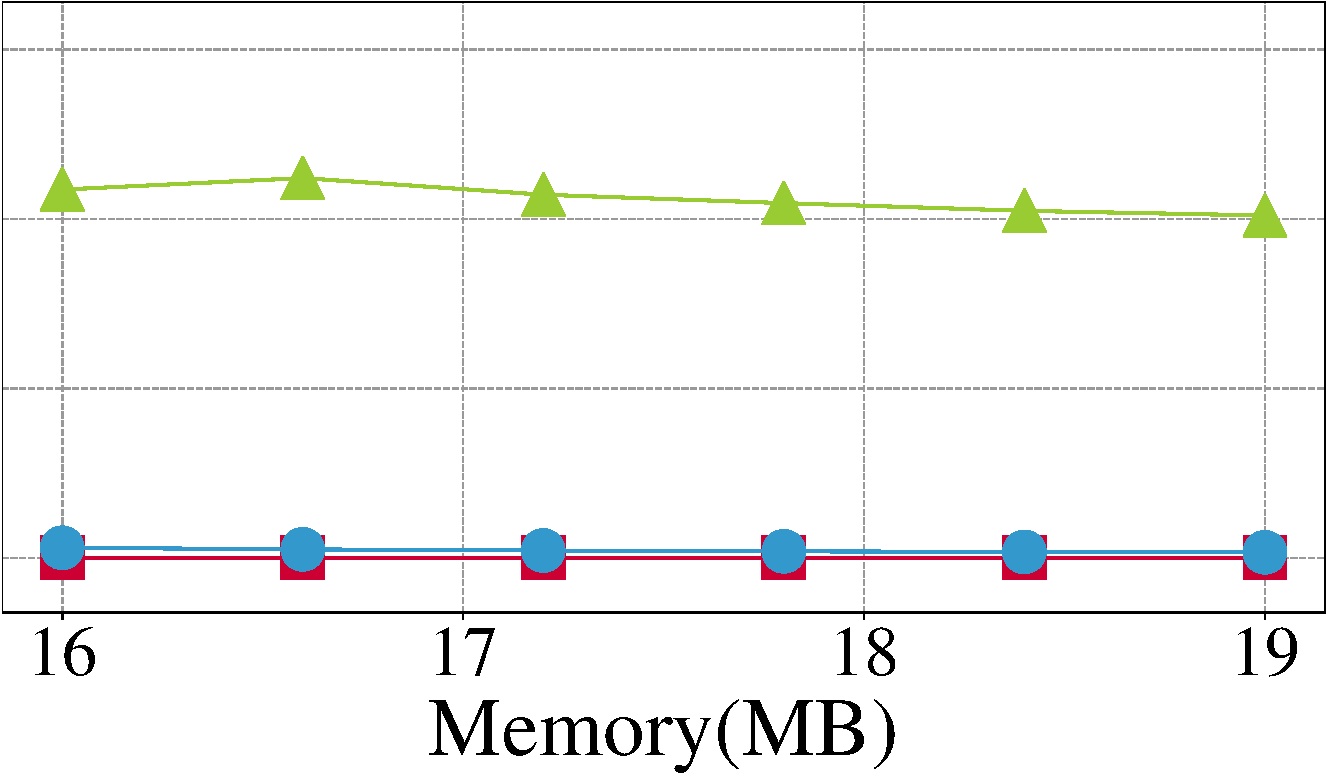
\includegraphics[width=0.95\textwidth, ]{Figures/per/per_are/per_ip_are-cropped.pdf}
		\end{center}
		}
		\postfig
		\adjustfigs
		\prefigcaption
		\label{per_are_ip}
		\postfigcaption
		\end{minipage}
	}
	%
	\subfigure[Web page]{
		\begin{minipage}[t]{0.225\textwidth}{
		\prefig
		\begin{center}		
		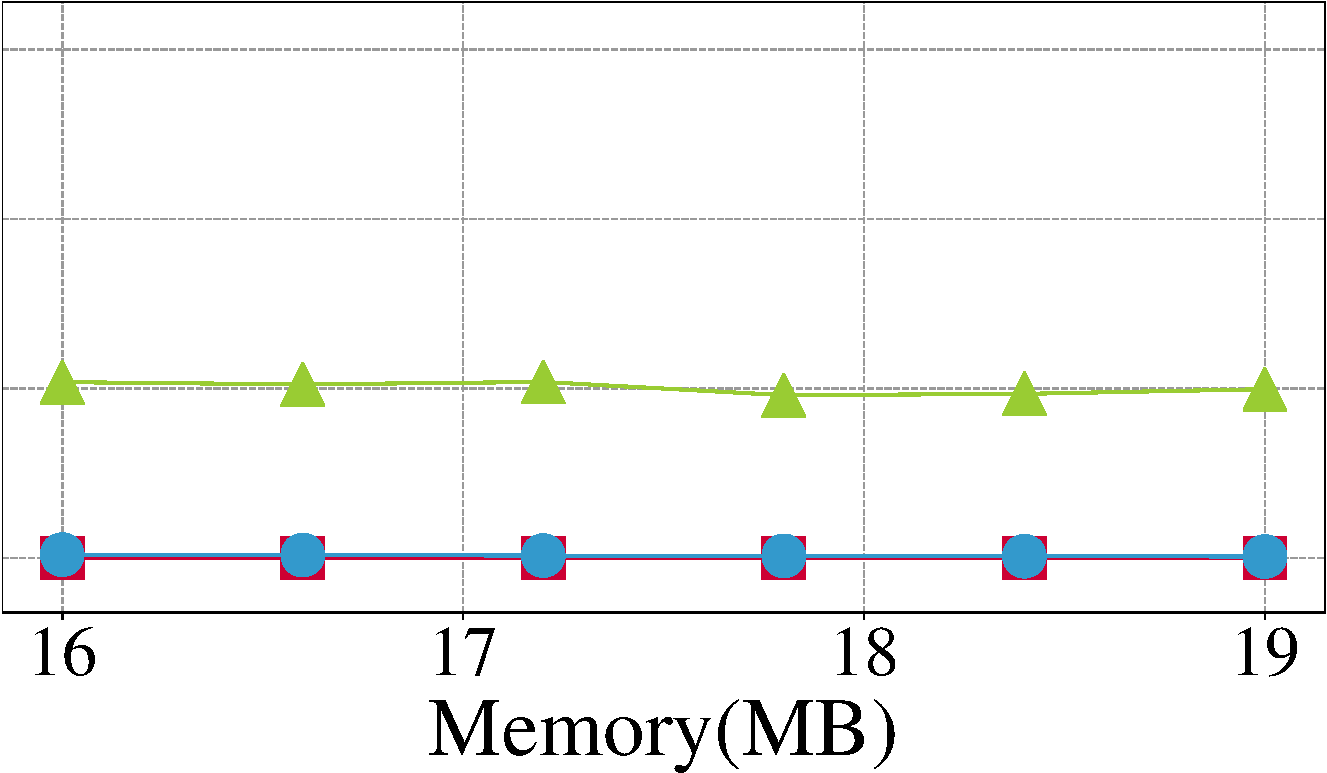
\includegraphics[width=0.95\textwidth, ]{Figures/per/per_are/per_web_are-cropped.pdf}\end{center}
		}
		\postfig 
		\adjustfigs
		\prefigcaption
		\label{per_are_web}
		\postfigcaption
		\end{minipage}
	}
	%
	\subfigure[Network dataset]{
		\begin{minipage}[t]{0.225\textwidth}{
		\prefig
		\begin{center}		
		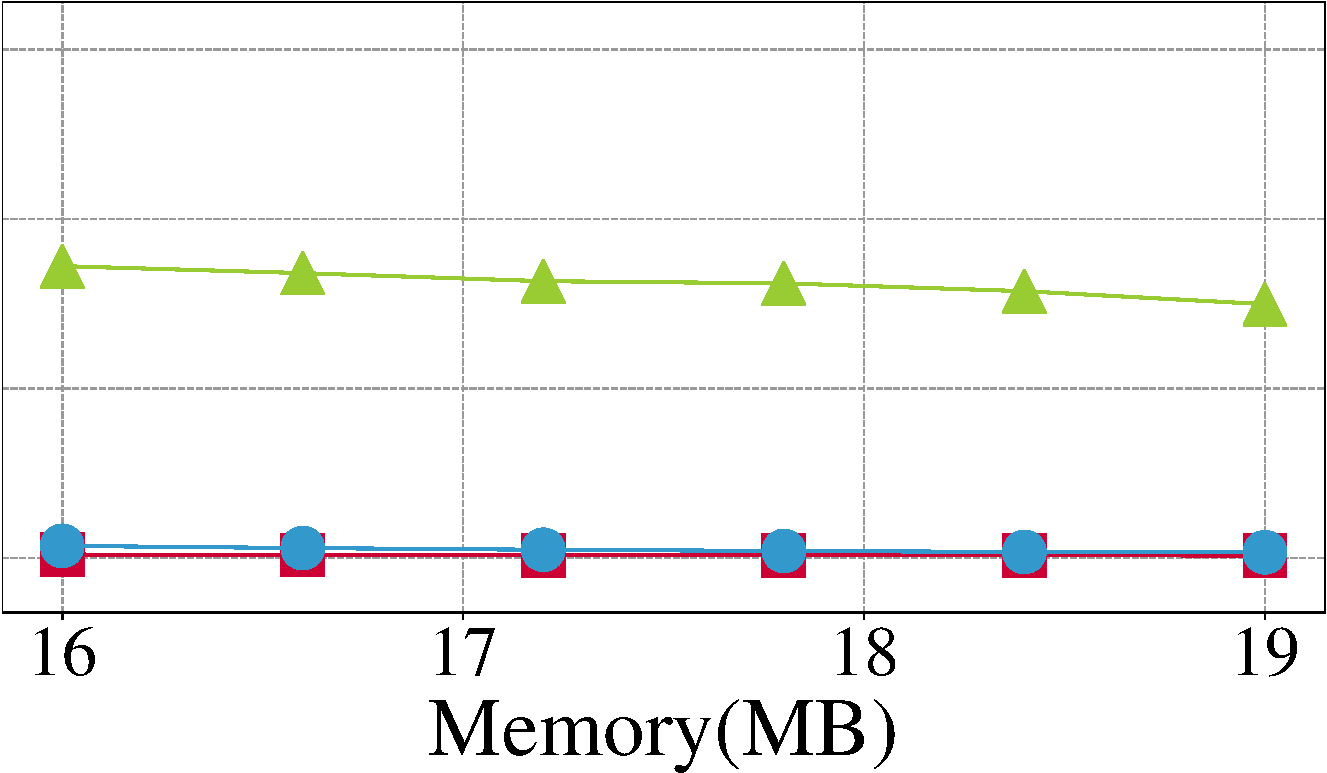
\includegraphics[width=0.95\textwidth, ]{Figures/per/per_are/per_net_are-cropped.pdf}
		\end{center}
		}
		\postfig 
		\adjustfigs
		\prefigcaption
		\label{per_are_net}
		\postfigcaption
		\end{minipage}
	}
	%
	\vvv \vvv
    \caption{ARE of finding \taskthree.}
	\label{per_are}
\end{figure*}

\begin{figure*}[!ht]
	\centering
	%
	\subfigure[Synthetic dataset]{
		\begin{minipage}[t]{0.255\textwidth}{
		\prefig
		\begin{center}
		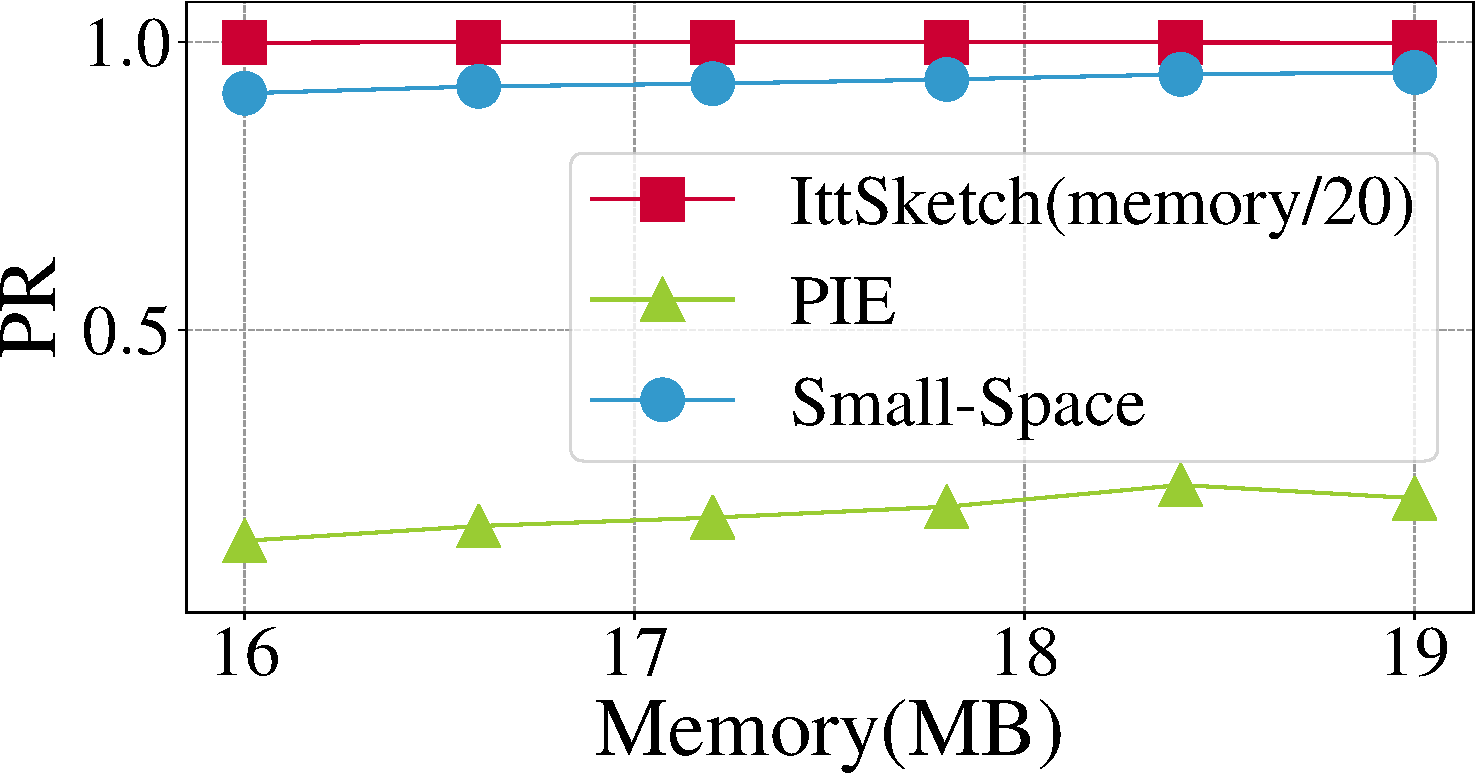
\includegraphics[width=0.95\textwidth, ]{Figures/per/per_pr/per_syn_pr-cropped.pdf}
		\end{center}
		}
		\postfig 
		\adjustfigs
		\prefigcaption
		\label{per_pr_syn}
		\postfigcaption
		\end{minipage}
	}
	%
	\subfigure[IP trace]{
		\begin{minipage}[t]{0.23\textwidth}{
		\prefig
		\begin{center}
		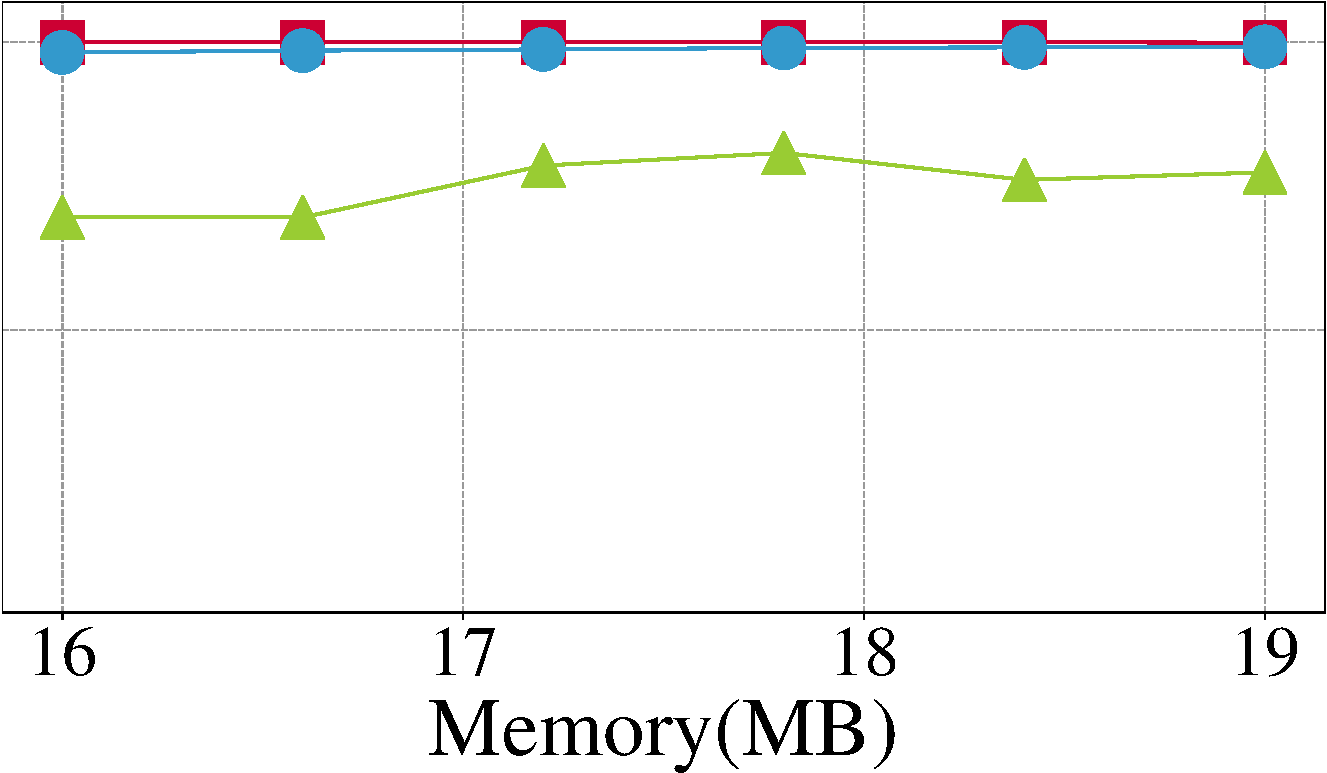
\includegraphics[width=0.95\textwidth, ]{Figures/per/per_pr/per_ip_pr-cropped.pdf}
		\end{center}
		}
		\postfig
		\adjustfigs
		\prefigcaption
		\label{per_pr_ip}
		\postfigcaption
		\end{minipage}
	}
	%
	\subfigure[Web page]{
		\begin{minipage}[t]{0.23\textwidth}{
		\prefig
		\begin{center}		
		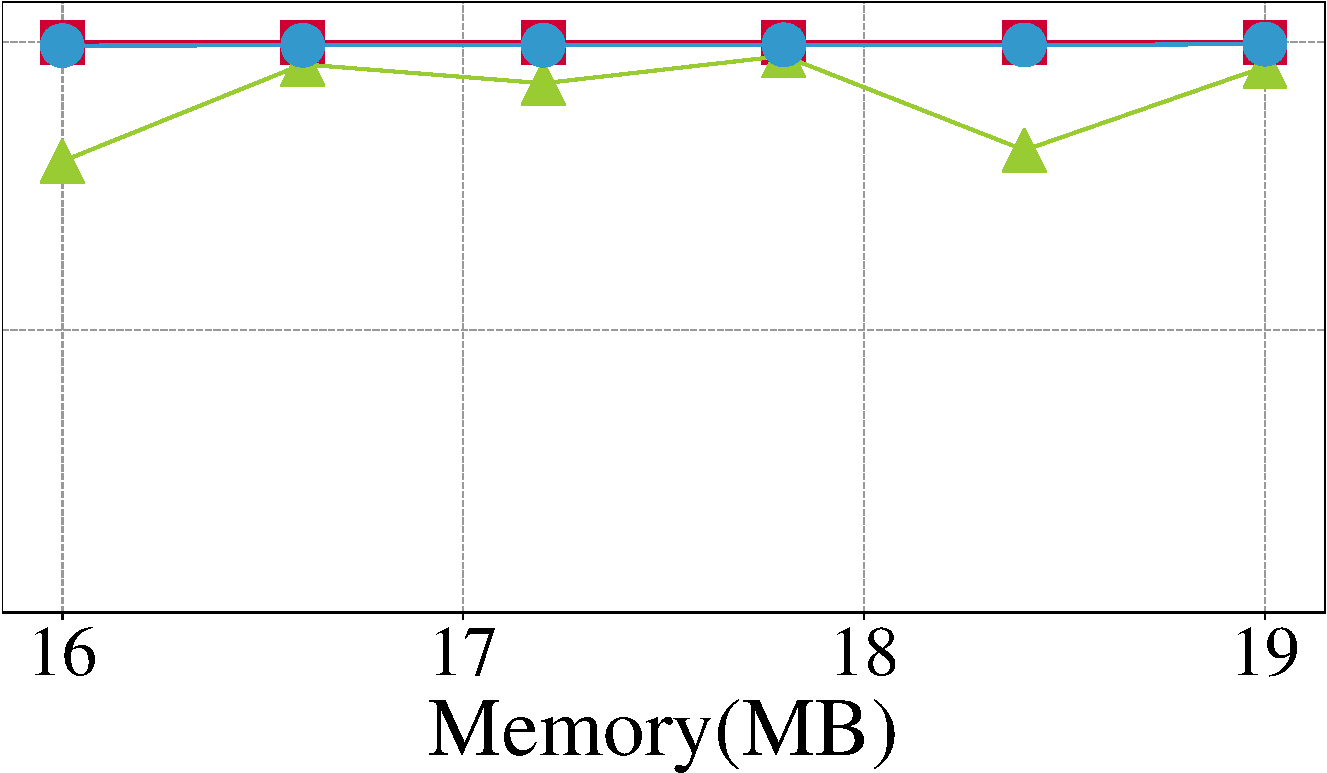
\includegraphics[width=0.95\textwidth, ]{Figures/per/per_pr/per_web_pr-cropped.pdf}
		\end{center}
		}
		\postfig 
		\adjustfigs
		\prefigcaption
		\label{per_pr_web}
		\postfigcaption
		\end{minipage}
	}
	%
	\subfigure[Network dataset]{
		\begin{minipage}[t]{0.23\textwidth}{
		\prefig
		\begin{center}		
		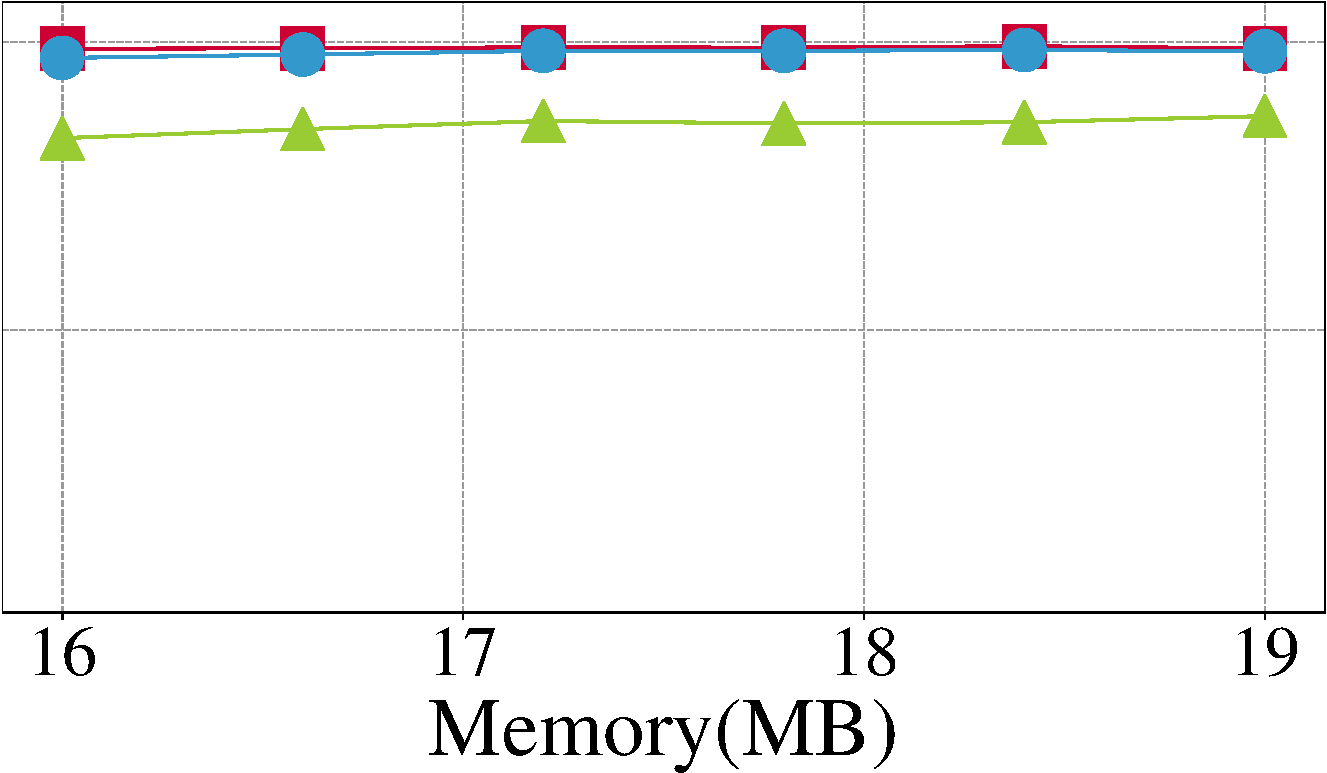
\includegraphics[width=0.95\textwidth, ]{Figures/per/per_pr/per_net_pr-cropped.pdf}
		\end{center}
		}
		\postfig 
		\adjustfigs
		\prefigcaption
		\label{per_pr_net}
		\postfigcaption
		\end{minipage}
	}
	%
	\vvv \vvv
    \caption{PR of finding \taskthree.}
	\label{per_pr}
\end{figure*}

\begin{figure*}[!ht]
	\centering
	%
	\subfigure[Synthetic dataset]{
		\begin{minipage}[t]{0.246126\textwidth}{
		\prefig
		\begin{center}
		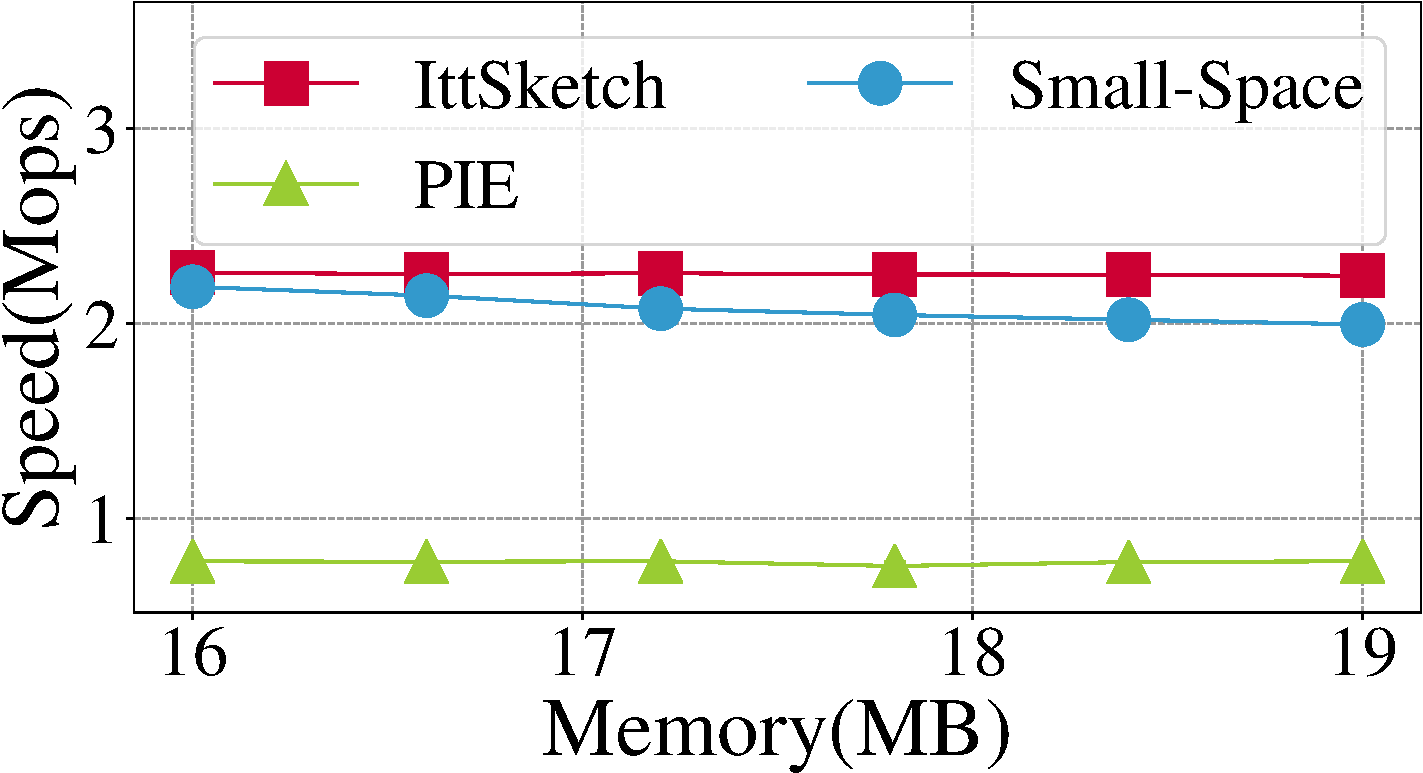
\includegraphics[width=0.95\textwidth, ]{Figures/per/per_speed/per_syn_speed-cropped.pdf}
		\end{center}
		}
		\postfig 
		\adjustfigs
		\prefigcaption
		\label{per_speed_syn}
		\postfigcaption
		\end{minipage}
	}
	%
	\subfigure[IP trace]{
		\begin{minipage}[t]{0.230622\textwidth}{
		\prefig
		\begin{center}
		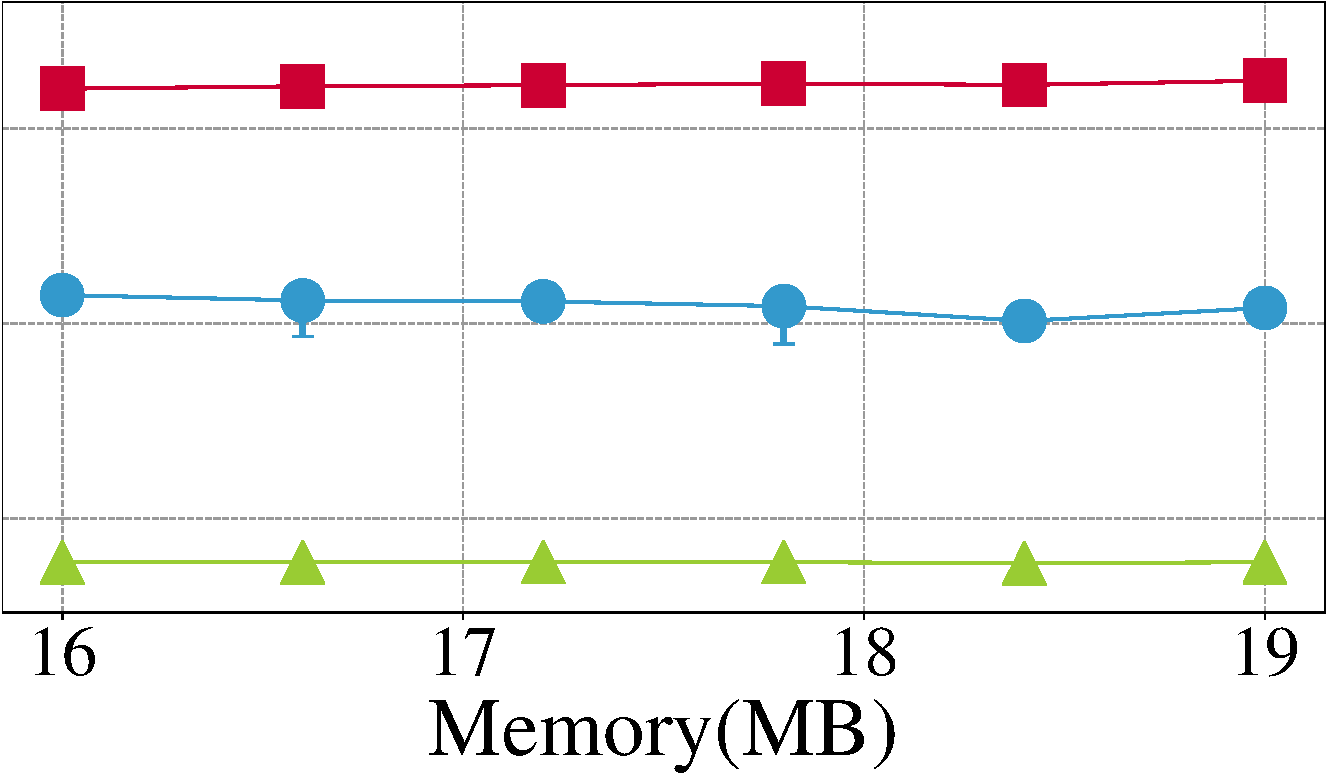
\includegraphics[width=0.95\textwidth, ]{Figures/per/per_speed/per_ip_speed-cropped.pdf}
		\end{center}
	    }
		\postfig
		\adjustfigs
		\prefigcaption
		\label{per_speed_ip}
		\postfigcaption
		\end{minipage}
	}
	%
	\subfigure[Web page]{
		\begin{minipage}[t]{0.230622\textwidth}{
		\prefig
		\begin{center}		
		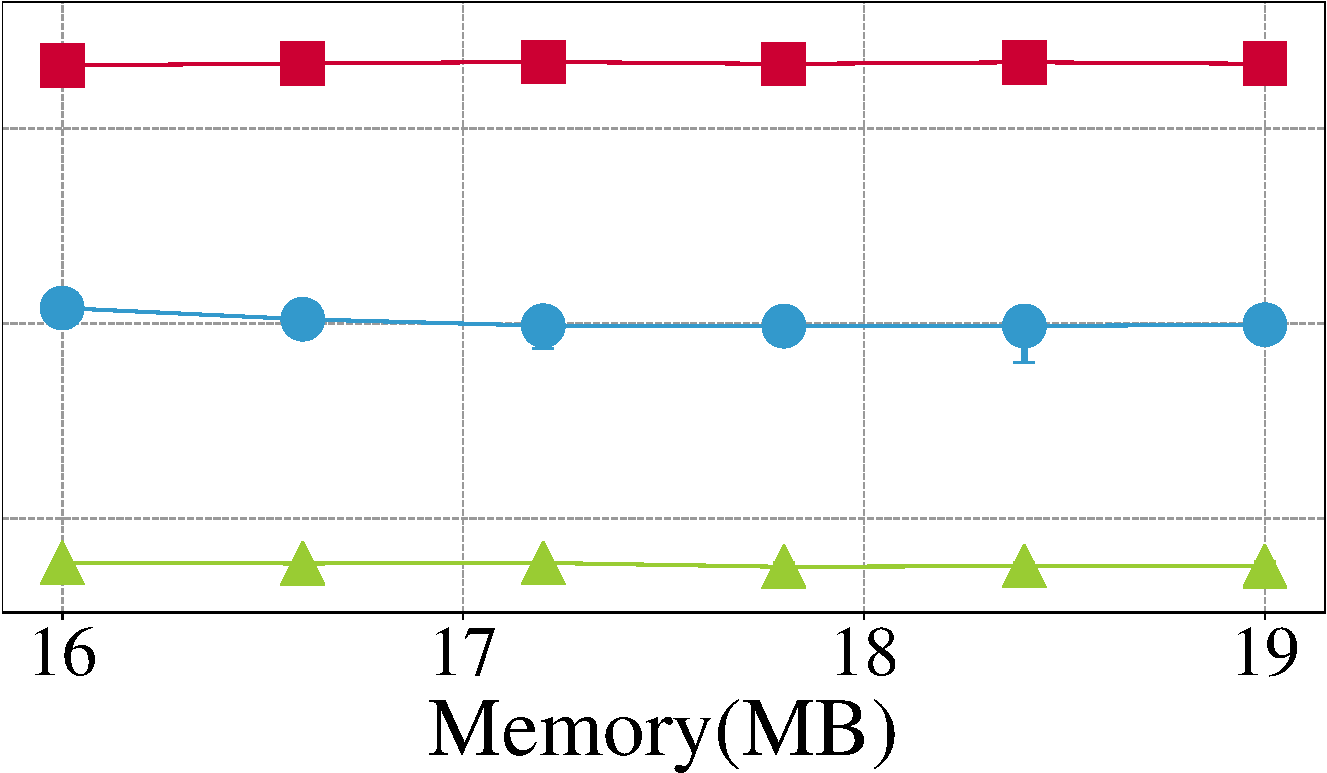
\includegraphics[width=0.95\textwidth, ]{Figures/per/per_speed/per_web_speed-cropped.pdf}
		\end{center}
		}
		\postfig 
		\adjustfigs
		\prefigcaption
		\label{per_speed_web}
		\postfigcaption
		\end{minipage}
	}
	%
	\subfigure[Network dataset]{
		\begin{minipage}[t]{0.230622\textwidth}{
		\prefig
		\begin{center}		
		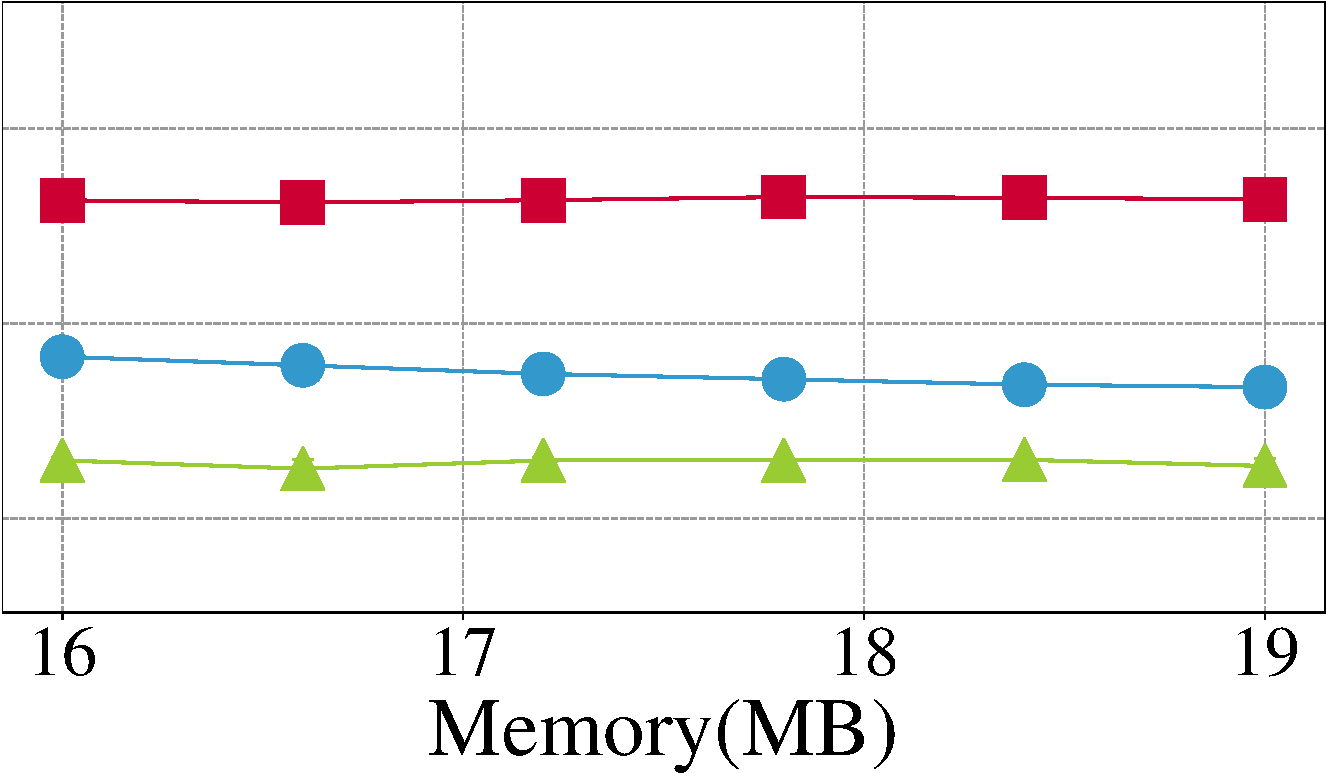
\includegraphics[width=0.95\textwidth, ]{Figures/per/per_speed/per_net_speed-cropped.pdf}
		\end{center}
		}
		\postfig 
		\adjustfigs
		\prefigcaption
		\label{per_speed_net}
		\postfigcaption
		\end{minipage}
	}
	%
	\vvv \vvv
    \caption{Speed of finding \taskthree.}
	\label{per_speed}
\end{figure*}	

%\presub
\subsection{Evaluation on Finding \tasktwo} %\postsub
\label{eva_two}

\noindent\textbf{Parameter Setting:}
%We compare three frameworks: \sketchname, \EHname and \Splittername. For each frameworks, we using CM Sketch, CM-CU Sketch and Count Sketch approaches.
%
%We compare 5 approaches: CM \sketchname, CM-CU \sketchname, Count \sketchname, \EHname {} and \Splittername.
%
%
%原则:抄袭:不能连续六个一样的单词。。。
We compare 4 algorithms: \sketchname, \supolf\cite{superspreader}, \suptlf\cite{superspreader}, and \supopen\cite{opensketch}.
Let $z$ be the number of hash functions for the Bloom filter. For \sketchname{}, we set $z=4$.
For \supolf, \suptlf{}, and \supopen, the parameters are set according to the recommendation of the authors.
In the experiment, we compare AAE, ARE, PR, CR, and insertion speed among the 4 algorithms.
The memory size ranges from 500KB to 750KB. Because other algorithms often spend much memory on the hash table or bitmap, more memory is required for the experiment. Also, we split the IP Trace Dataset into 4 sub-datasets.
			
%% why different memory size for different interest...
%% cherry picker...

\noindent\textbf{ARE (Figure~\ref{sup_are_ip}-\ref{sup_are_ip8}):}
We find that the ARE of \sketchname{} is around 31 times, 30 times, and 18 times lower than \supolf, \suptlf{}, and \supopen{}, respectively.
			
\noindent\textbf{PR (Figure~\ref{sup_pr_ip}-\ref{sup_pr_ip8}):}
We find that \sketchname{} achieves a PR above 0.99 when the memory is more than 500KB. The PR of \sketchname{} is around 4.1 times, 3.4 times, and 1.9 times higher than \supolf, \suptlf{}, and \supopen{}, respectively.
			
			
\noindent\textbf{Speed (Figure~\ref{sup_speed_ip}-\ref{sup_speed_ip8}):}
We find that, on IP Trace datasets, the insertion speed of \sketchname{} is slower than \supolf{} and \suptlf{} but is faster than \supopen{}.

\noindent\textbf{AAE (Figure~\ref{sup_aae_ip}-\ref{sup_aae_ip8}) in Appendix \ref{app:fig}:}
We find that the AAE of \sketchname{} is around 14 times, 13.3 times, and 40 times lower than \supolf, \suptlf{}, and \supopen{}, respectively.

\noindent\textbf{CR (Figure~\ref{sup_cr_ip}-\ref{sup_cr_ip8}) in Appendix \ref{app:fig}:}
We find that the CR of \sketchname{} is around 1.4 times, 1.6 times, and 1.8 times higher than \supolf, \suptlf{}, and \supopen{}, respectively.

\noindent\textbf{Summary:} 
1) \sketchname{} is more accurate than other algorithms because other algorithms often spend much memory on the hash table or bitmap, which makes them unable to count items precisely.

2) Our results show that \sketchname{} achieves both high recall rate and high precision rate. Though \supolf{} and \suptlf{} report more correct instances than \supopen{}, they also report more wrong instances due to their low sample rate, making their precision rate lower than 0.03. 
\presub %\vvv
\subsection{Evaluation on Finding \taskthree} %\postsub
\label{eva_three}

\noindent\textbf{Parameter Setting:}
%We compare three frameworks: \sketchname, \EHname and \Splittername. For each frameworks, we using CM Sketch, CM-CU Sketch and Count Sketch approaches.
%
%We compare 5 approaches: CM \sketchname, CM-CU \sketchname, Count \sketchname, \EHname {} and \Splittername.
%
We compare 3 algorithms: \sketchname, \perpie\cite{persisitem}, and \perss\cite{smallspace}.
Let $z$ be the number of hash functions for the Bloom filter. For \sketchname{}, we set $z=3$.
For \perpie{} and \perss, the parameters are set according to the recommendation of the authors.
In the experiment, we compare AAE, ARE, PR, CR, and insertion speed among the 3 algorithms.
The memory size ranges from 16MB to 19MB. We choose this range because \perpie{} cannot report any interesting items on the synthetic dataset if memory size is less than 16MB. Also, we set the memory size of \sketchname{} to $1/20$ of the memory size of the other algorithms when we compare AAE, ARE, PR, and CR. 
We do this because when memory size is more than 16MB, the AAE and ARE of \sketchname{} are 0, and the CR and PR of \sketchname{} are 1. To compare these algorithms more conveniently, we reduce the memory size of \sketchname.
			
			
\noindent\textbf{ARE (Figure~\ref{per_are_syn}-\ref{per_are_net}):}
We find that, on three real-world datasets, the ARE of \sketchname{} is around 771 times and 50212 times lower than \perss{} and \perpie. On the synthetic dataset, the ARE of \sketchname{} is around 115 times and 1655 times lower than \perss{} and \perpie.  


\noindent\textbf{PR (Figure~\ref{per_pr_syn}-\ref{per_pr_net}):}
We find that, on three real-world datasets, the PR of \sketchname{} is around 1.01 times and 1.23 times higher than \perss{} and \perpie. On the synthetic dataset, the PR of \sketchname{} is around 1.08 times and 6 times higher than \perss{} and \perpie.  
			
			
\noindent\textbf{Speed (Figure~\ref{per_speed_syn}-\ref{per_speed_net}):}
We find that the insertion speed of \sketchname{} is around 1.4 times and 4 times faster than \perss{} and \perpie{} on three real-world datasets and one synthetic dataset.

\noindent\textbf{AAE (Figure~\ref{per_aae_syn}-\ref{per_aae_net}) in Appendix \ref{app:fig}:}
We find that, on three real-world datasets, the AAE of \sketchname{} is around 698 times and 53543 times lower than \perss{} and \perpie. On the synthetic dataset, the AAE of \sketchname{} is around 167 times and 6095 times lower than \perss{} and \perpie. 

\noindent\textbf{CR (Figure~\ref{per_cr_syn}-\ref{per_cr_net}) in Appendix \ref{app:fig}:}
We find that, on three real-world datasets, the CR of \sketchname{} is around 1.03 times and 33 times higher than \perss{} and \perpie. On the synthetic dataset, the CR of \sketchname{} is around 1.05 times and 33 times higher than \perss{} and \perpie.  

\noindent\textbf{Summary:}
%
1) Although the memory size of \sketchname{} is only $1/20$ of the other algorithms, it still performs much better. The ARE of \sketchname{} is lower than 0.005 when its memory size is more than 800KB on three real-world datasets and one synthetic dataset.

2) The PR and CR of \sketchname{} are often more than 0.99 when its memory size is more than 800KB on three real-world datasets and one synthetic dataset. The PR and CR of \perss{} are often more than 0.95 when its memory size is more than 16MB on three real-world datasets and one synthetic dataset. However, the CR of \perpie{} is often lower than 0.2 because it wastes much of the space to record the items in every period.

3) \sketchname{} can achieve higher insertion speed compared to \perss{} and \perpie. Also, \sketchname{} will not be slower when its memory use increases. In contrast, \perss{} slows down as memory use increases.
{\color{reviewA}
\presub
\subsection{Evaluation on Distributions and Arrival Orders} \postsub
\label{eva_data}

\begin{figure}[!ht]
	\centering
	\subfigure[Impact of dataset distribution]{
		\begin{minipage}[t]{0.22\textwidth}{
			\prefig
			\begin{center}
			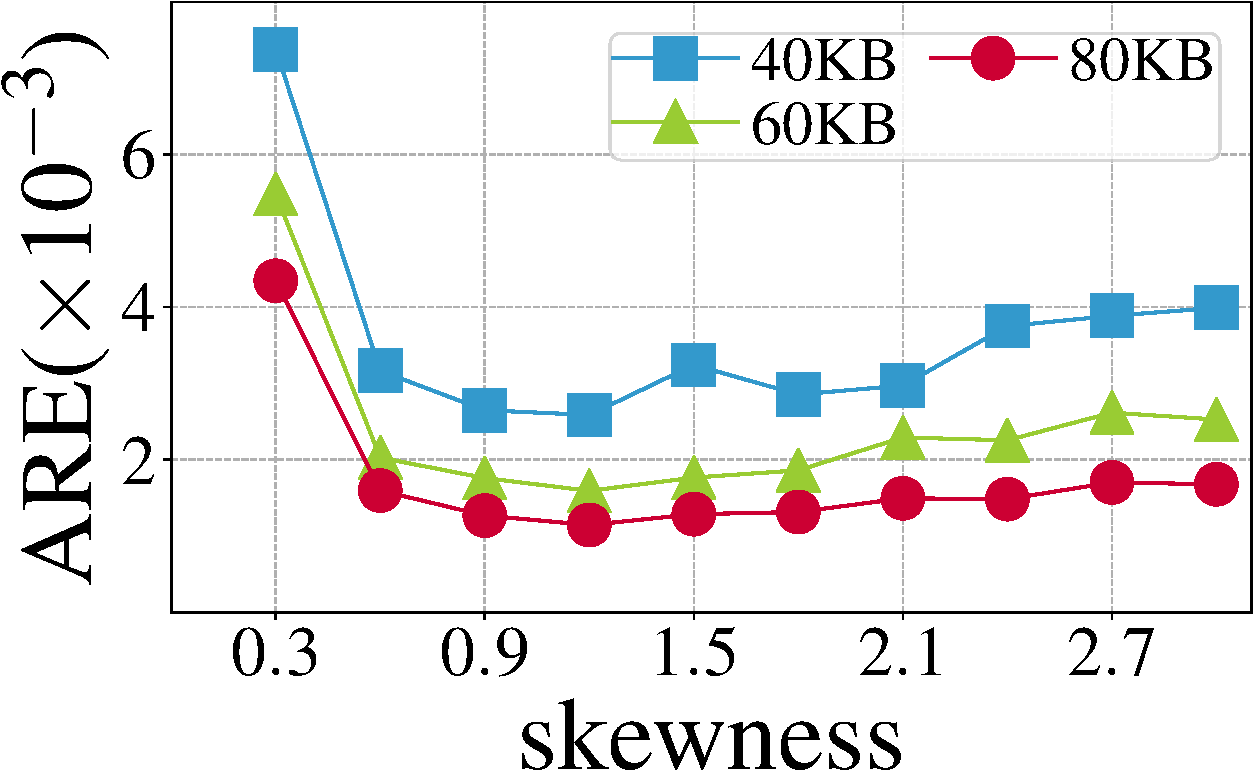
\includegraphics[width=\textwidth, ]{Figures/dataset/skew_out_are-cropped.pdf}
			\end{center}}
			\postfig 
			\adjustfigs
			\prefigcaption
			\label{skew_are}
			\postfigcaption
		\end{minipage}
	}
	\subfigure[Impact of arrival order]{
		\begin{minipage}[t]{0.22\textwidth}{
		    \prefig
			\begin{center}
			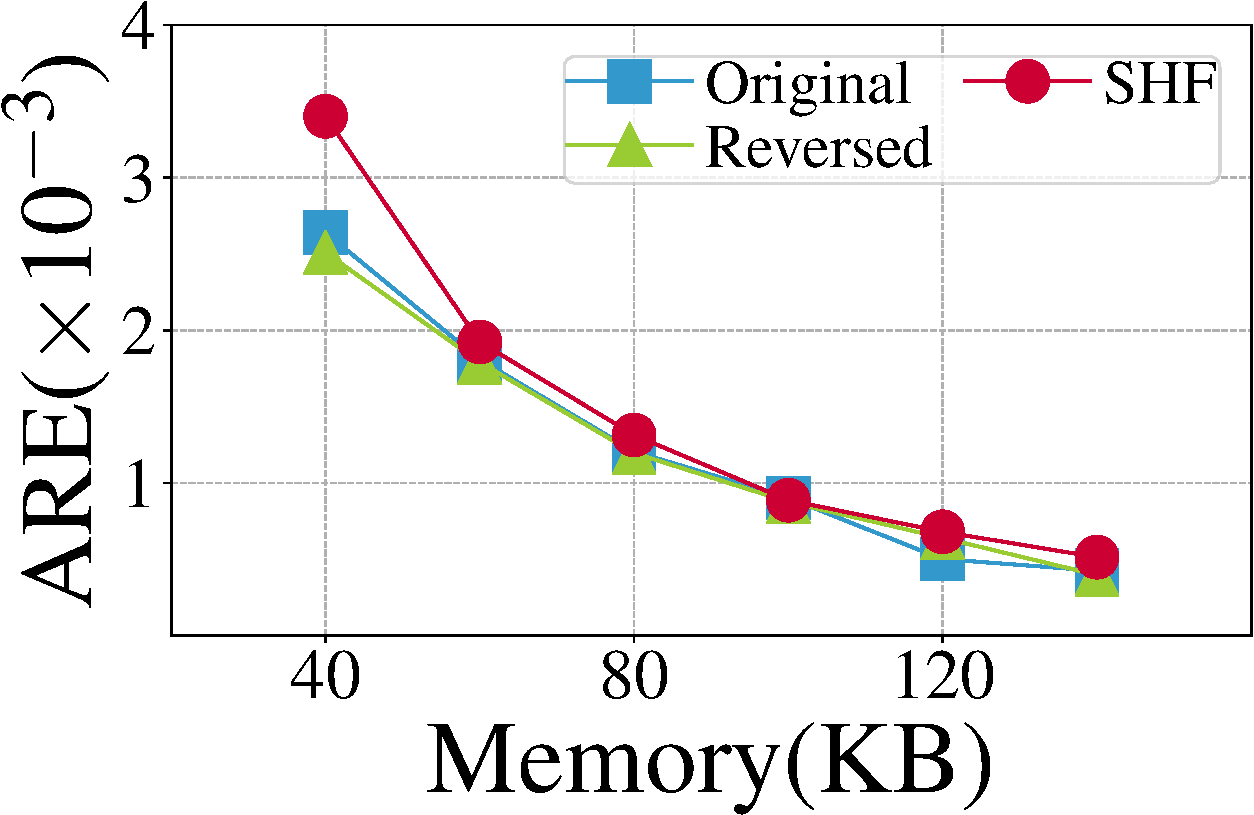
\includegraphics[width=\textwidth, ]{Figures/dataset/order_out_are-cropped.pdf}
			\end{center}}
			\postfig
			\adjustfigs
			\prefigcaption
			\label{order_are}
			\postfigcaption
		\end{minipage}}
	\vvv \vvv
    \caption{Accuracy vs. skewness and item arrival order. Given a dataset, ``SHF'' refers to that the Second Half of items go First.}
	\label{dataset}
\end{figure}

In this subsection, we show how the dataset distribution and the arrival order of items affect the accuracy of PRI.

\noindent\textbf{Parameter Setting:}
We use synthetic datasets whose skewness varies from 0.3 to 3.0 to show the impact of dataset distribution to InterestSketch. We use the dataset whose skewness is 1.5 and three different orders to show the impact of the arrival order of items. Three different orders are the original order, the reversed order, and the Second Half First (SHF).
%
In this experiment, we plot the change of ARE of InterestSketch to show the impact.
The size of memory used ranges from 40KB to 140KB. We choose this range because using small memory can clearly expose the impact.

\noindent\textbf{Impact of dataset distribution (Figure~\ref{skew_are}):}
Our results show that the ARE of \sketchname{} is often lower than 0.01, and changes a little bit, especially when skewness is larger than 0.6.

\noindent\textbf{Impact of arrival orders (Figure~\ref{order_are}):}
Our results show that arrival orders indeed make some effects on the ARE of our \sketchname, but the effect is also not significant.
Because PRI replaces the minimum counter with a probability, the fluctuation of ARE in a certain range is reasonable.
}

{\color{reviewD}
\presub
\subsection{Extending SS and USS for Other Tasks} %\postsub
\label{eva_other}

\noindent\textbf{Parameter Setting:}
In this subsection, we use Unbiased SS\cite{unbiasedsketch} and SS\cite{spacesaving} to address the other three kinds of tasks.
We use \textit{IP Trace Dataset} to evaluate because only IP Trace Dataset can be used for finding Super-Spreaders.
			
\begin{figure*}[!ht]
	\centering
	\subfigure[CR of Finding \taskfour]{
		\begin{minipage}[t]{0.23\textwidth}{
			\prefig
			\begin{center}
			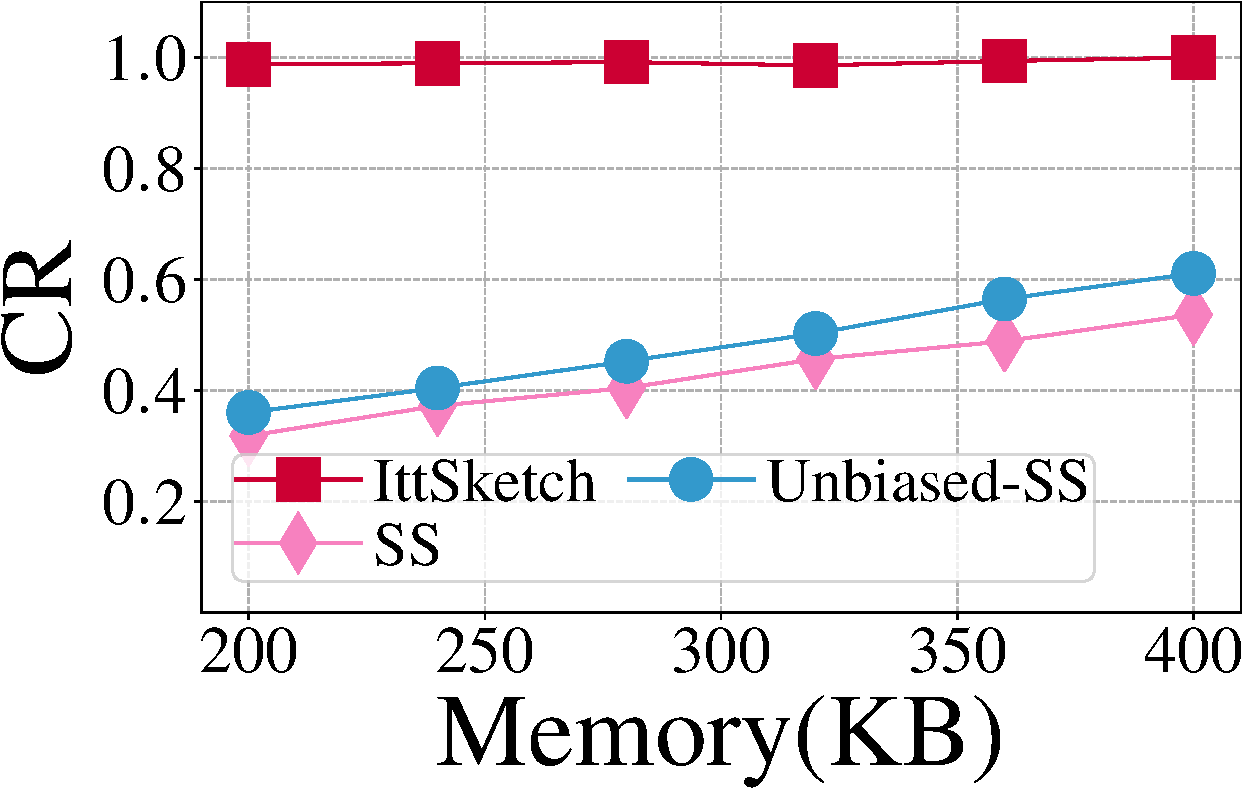
\includegraphics[width=\textwidth, ]{Figures/other/other_cha_cr-cropped.pdf}
			\end{center}}
			\postfig 
			\adjustfigs
			\prefigcaption
			\label{other_cha_cr}
			\postfigcaption
		\end{minipage}
	}
	\subfigure[PR of Finding \taskfour]{
		\begin{minipage}[t]{0.23\textwidth}{
		    \prefig
			\begin{center}
			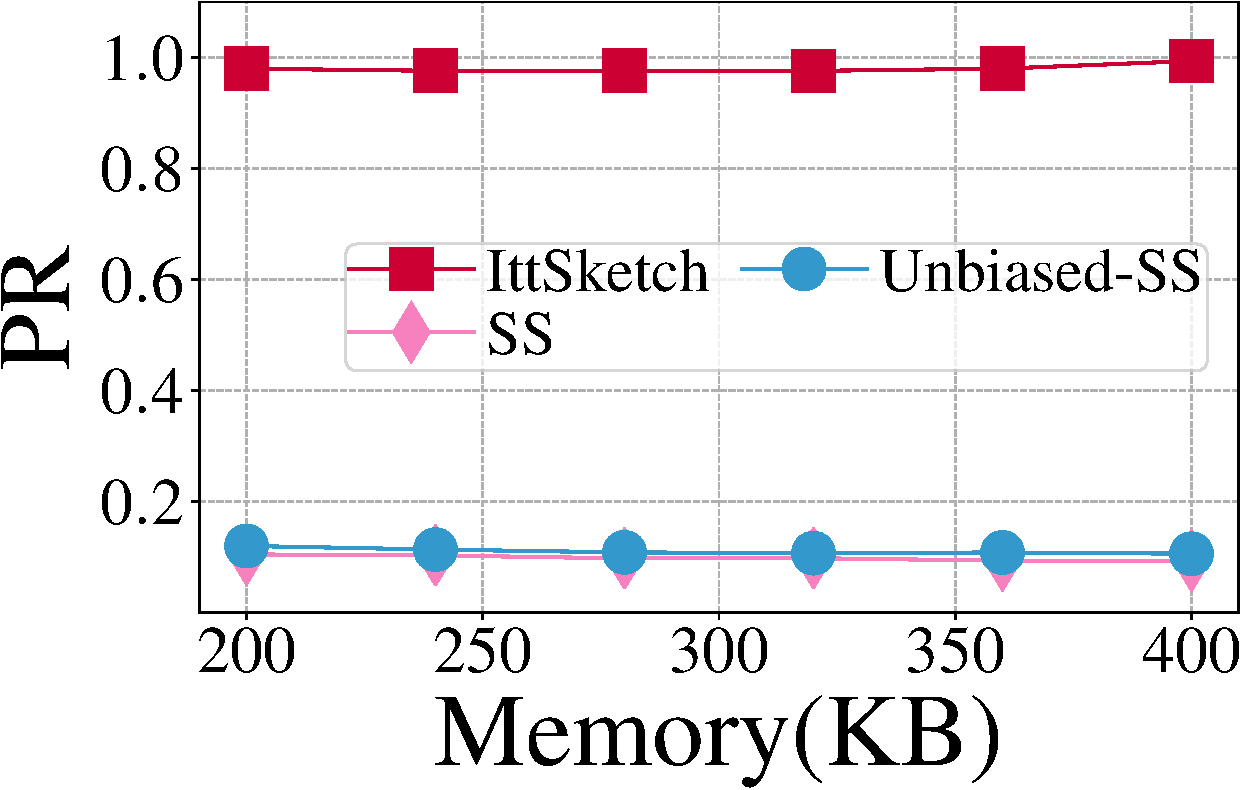
\includegraphics[width=\textwidth, ]{Figures/other/other_cha_pr-cropped.pdf}
			\end{center}}
			\postfig
			\adjustfigs
			\prefigcaption
			\label{other_cha_pr}
			\postfigcaption
		\end{minipage}}
	\subfigure[ARE of Finding \tasktwo]{
		\begin{minipage}[t]{0.23\textwidth}{
			\prefig
			\begin{center}
			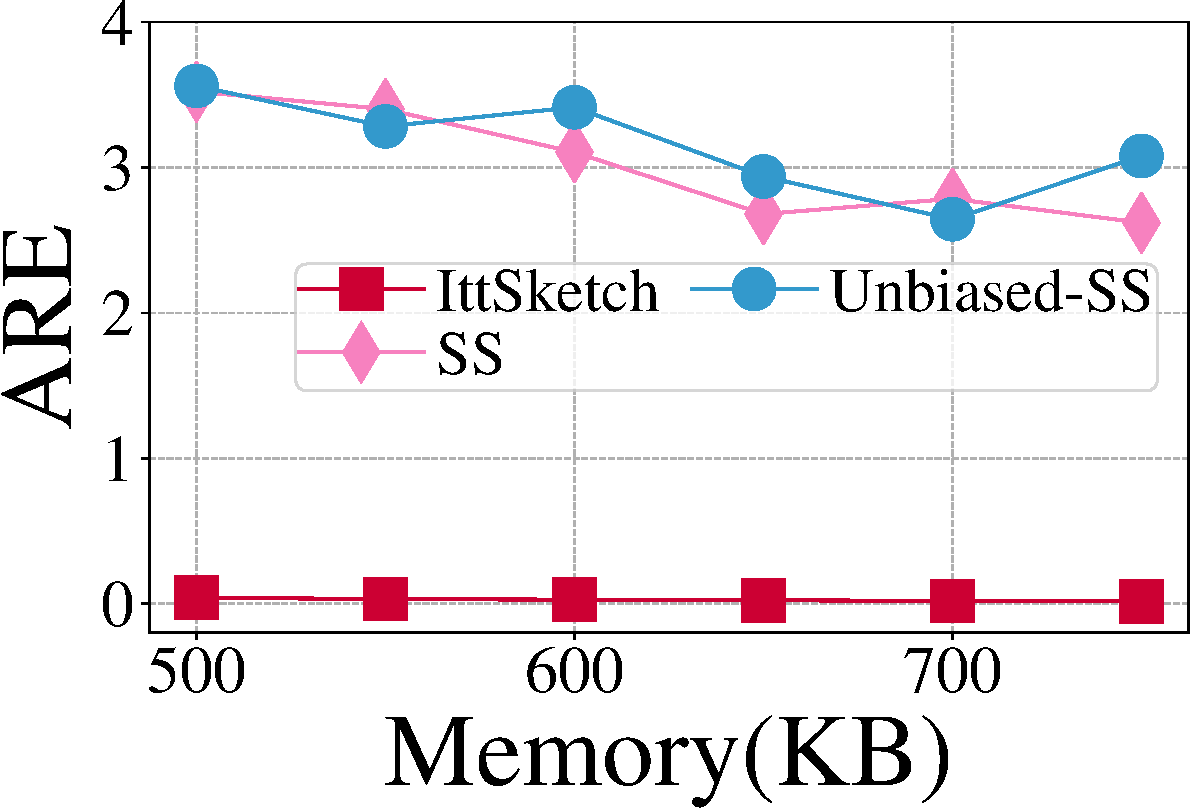
\includegraphics[width=\textwidth, ]{Figures/other/other_sup_are-cropped.pdf}
			\end{center}}
			\postfig 
			\adjustfigs
			\prefigcaption
			\label{other_sup_are}
			\postfigcaption
		\end{minipage}
	}
	\subfigure[ARE of Finding \taskthree]{
		\begin{minipage}[t]{0.23\textwidth}{
		    \prefig
			\begin{center}
			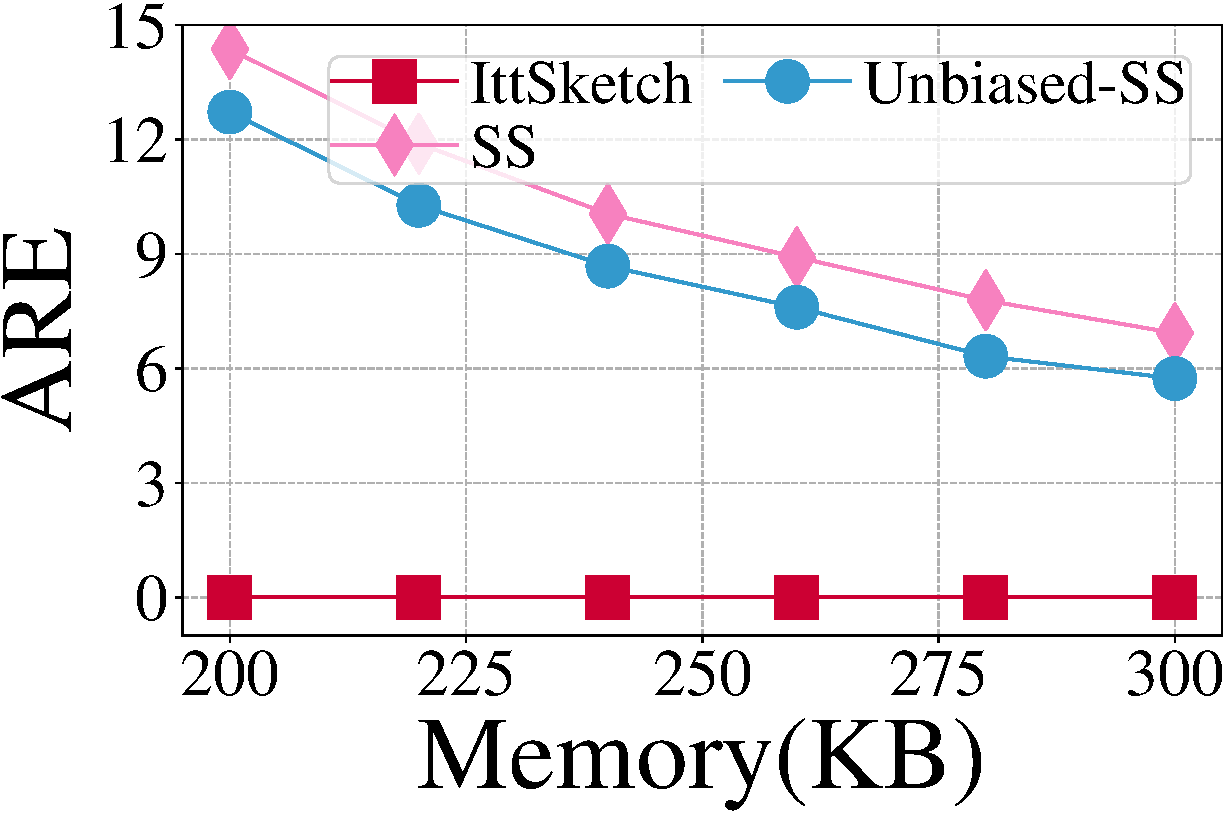
\includegraphics[width=\textwidth, ]{Figures/other/other_per_are-cropped.pdf}
			\end{center}}
			\postfig
			\adjustfigs
			\prefigcaption
			\label{other_per_are}
			\postfigcaption
		\end{minipage}}
	\vvv \vvv
    \caption{Accuracy comparison of InterestSketch, SS, and USS for other three tasks.}
	\label{other}
\end{figure*}

\begin{figure*}[!ht]
	\centering
	\subfigure[Latency of Finding \taskone]{
		\begin{minipage}[t]{0.23\textwidth}{
			\prefig
			\begin{center}
			\includegraphics[width=\textwidth, ]{Figures/latency/fre_ip_latency-cropped.pdf}
			\end{center}}
			\postfig 
			\adjustfigs
			\prefigcaption
			\label{fre_ip_latency}
			\postfigcaption
		\end{minipage}
	}
	\subfigure[Latency of Finding \taskfour]{
		\begin{minipage}[t]{0.23\textwidth}{
		    \prefig
			\begin{center}
			\includegraphics[width=\textwidth, ]{Figures/latency/cha_ip_latency-cropped.pdf}
			\end{center}}
			\postfig
			\adjustfigs
			\prefigcaption
			\label{cha_ip_latency}
			\postfigcaption
		\end{minipage}
	}
	\subfigure[Latency of Finding \tasktwo]{
		\begin{minipage}[t]{0.23\textwidth}{
			\prefig
			\begin{center}
			\includegraphics[width=\textwidth, ]{Figures/latency/sup_ip_latency-cropped.pdf}
			\end{center}}
			\postfig 
			\adjustfigs
			\prefigcaption
			\label{sup_ip_latency}
			\postfigcaption
		\end{minipage}
	}
	\subfigure[Latency of Finding \taskthree]{
		\begin{minipage}[t]{0.23\textwidth}{
		    \prefig
			\begin{center}
			\includegraphics[width=\textwidth, ]{Figures/latency/per_ip_latency-cropped.pdf}
			\end{center}}
			\postfig
			\adjustfigs
			\prefigcaption
			\label{per_ip_latency}
			\postfigcaption
		\end{minipage}
	}
	%\vvv \vvv
    \caption{Latency of four tasks.}
	\label{latency}
\end{figure*}
			
\noindent\textbf{CR and PR of Finding \taskfour{} (Figure~\ref{other_cha_cr}-\ref{other_cha_pr}):}
We can find that, the CR of \sketchname{} is around 2.67 times and 2.45 times higher than SS and Unbiased SS. According to Figure \ref{other_cha_pr}, the PR of \sketchname{} is around 9.33 times and 8.17 times higher than SS and Unbiased SS.

\noindent\textbf{ARE of Finding \tasktwo{} (Figure~\ref{other_sup_are}):}
We find that, the ARE of \sketchname{} is around 115.5 times and 126.7 times higher than SS and Unbiased SS. The ARE of \sketchname{} is often lower than 0.04, while the ARE of SS and Unbiased SS is often higher than 2.6.

\noindent\textbf{ARE of Finding \taskthree{} (Figure~\ref{other_per_are}):}
Our results show that the ARE of \sketchname{} is around 2347 times and 2000 times higher than SS and Unbiased SS. The ARE of \sketchname{} is often lower than 0.006, while the ARE of SS and Unbiased SS is often higher than 5.

\noindent\textbf{Summary:}
%
1) 
The ARE of SS and Unbiased SS are often higher than 2.6.
Similar to the performance on finding frequent items, the ARE of SS and Unbiased SS are often much higher than that of \sketchname{} on other three tasks.
Because they cannot accurately record the frequency of frequent items, they also can not perform well on other tasks which is highly related to item frequencies.
}

%\vspace{-0.07in}
{\color{reviewD}
\presub
\subsection{Evaluation on Latency} %\postsub
\label{eva_latency}

We use IP Trace Dataset to evaluate latency. Parameters setting is the same as that of each previous task.

\noindent\textbf{Latency of four tasks (Figure~\ref{fre_ip_latency}-\ref{per_ip_latency}):}
According to the results, the latency of our \sketchname{} is often smaller than other algorithms. For our \sketchname{}, the latency of finding Super-Spreaders is similar to that of finding frequent items and finding heavy changes. The latency of finding persistent items is higher because we need to periodically clear the Bloom filter.
Besides, to achieve head-to-head comparison, we use more memory in finding persistent items than other tasks, because other algorithms on finding persistent items, like PIE, cannot work if memory size is less than 16MB.
}
\presub 
\subsection{Limitations of Our Final Version} %\postsub
\label{eva_def}

The above experimental results show that the final version of \sketchname{} can achieve high accuracy with small memory. However, the final version cannot guarantee that it will report all the interest items correctly even with larger amount of memory. We can only claim that as the memory increases, the final version has a higher probability to be correct. In contrast, the basic version of \sketchname{} can record all the flows if it has enough memory. Though it may use more memory and be slower, its correctness can be guaranteed when the memory size is large enough.
When compared with the Unbiased SpaceSaving \cite{unbiasedsketch}, another shortcoming of InterestSketch is that the InterestSketch is biased.
However, InterestSketch achieves 1820$\sim$2576 smaller error rate than the Unbiased SpaceSaving (see Figure \ref{fre_are}).
